%
% Author:  Klára Pacalová
% E-mail:  pacalkla@fel.cvut.cz
% Date:    24.02.2018 11:03
%
\documentclass[twoside]{article}
\usepackage[a4paper]{geometry}
\geometry{verbose,tmargin=2.5cm,bmargin=2cm,lmargin=2cm,rmargin=2cm}
\usepackage{fancyhdr}
\pagestyle{fancy}
\usepackage{dirtree} %directory tree visualisation
\usepackage[utf8]{inputenc}
\usepackage[czech]{babel}
\usepackage{siunitx}
\usepackage{listings}
\usepackage{graphicx} %graphics files inclusion
\usepackage{amsmath} %advanced maths
\usepackage{amssymb} %additional math symbols
% nastavení pisma a češtiny
\usepackage{lmodern}
\usepackage[T1]{fontenc}
\usepackage{float}
\usepackage{xcolor}
\usepackage{authblk}
\graphicspath{{../Images/}}
\usepackage{titling}

% odkazy
\usepackage{url}

% vícesloupcové tabulky
\usepackage{multirow}

% automatická konverze schematu
\usepackage{pppfig}

% odkazy a záložky
\usepackage[unicode=true, bookmarks=true,bookmarksnumbered=true,
bookmarksopen=false, breaklinks=false,pdfborder={0 0 0},
pdfpagemode=UseNone,backref=false,colorlinks=true] {hyperref}

% smaz aktualni page layout
\fancyhf{}

 %zapati
\fancyhf[FC]{\thepage}

% nastavi novou stranku u sekce
\newcommand{\sekce}[1]{\clearpage \section{#1}}
\newcommand{\nadpis}[1]{\newpage \section*{#1}}

% Maple Output
\definecolor{MapleBlue}{rgb}{0,0,1}
\def\MapleOutput#1{{\begin{center}\begin{math}\color{MapleBlue}{#1}\end{math}\end{center}}}

% titulni strana
\begin{document}

% údaje o autorovi
\title{Analogový přeladitelný filtr se zesilovači OTA}
\author{Klára Pacalová}

% titulni strana
\pagenumbering{roman}

% zahlavi
\fancyhf[HC]{\bfseries\leftmark}

\begin{titlepage}
    \begin{center}
    
        
\includegraphics[width=0.5\textwidth]{logo_FEL_cb.jpg}
            
        \vspace*{3cm}
 	
        \Large Bakalářská práce \\
        \vspace*{1.5cm}
        \Huge
        \textbf{Analogový přeladitelný filtr se zesilovači OTA}
 
        \vspace{1cm}

        \Large{Klára Pacalová}
 
        \vfill
 
        \vspace{0.8cm}
 		
        \Large
 		Vedoucí práce: doc. Dr. Ing. Jiří Hospodka\\
    		\large Katedra teorie obvodů\\
		
		\vspace{1.5cm}
		        
		\large Praha, Prosinec 2019
 
    \end{center}
\end{titlepage}
\thispagestyle{empty} 
\nadpis{}
\vspace{18cm}

Prohlašuji, že jsem bakalářskoupráci na téma Analogový  přeladitelný filtr se zesilovači OTA vypracovala pod vedením vedoucího bakalářské práce samostatně za použití v práci uvedených pramenů a literatury. Dále prohlašuji, že tato bakalářská práce nebyla využita k získání jiného nebo stejného titulu.\\
\\
\\
\\
V Praze dne \today \hfill \hfill ....................................................

\thispagestyle{empty} 
\nadpis{}
\vfill

Vysokoškolská závěrečná práce je dílo chráněné autorským zákonem. Je možné pořizovat z něj na své náklady a pro svoji osobní potřebu výpisy, opisy a rozmnoženiny. Jeho využití musí být v souladu s autorským zákonem a citační etikou.\\

\noindent A university thesis is a work protected by the Copyright Act. Extracts, copies and transcripts of the thesis are allowed for personal use only and at one's own expense. The use of thesis should be in compliance with the Copyright Act and the citation ethics.\\

\noindent \textsuperscript{\textcopyright} Klára Pacalová, 2020\\
Fakulta elektrotechnická\\
České vysoké učení technické v Praze\\
Technická 2\\
160 00 Praha 6\\
Česká republika
\thispagestyle{empty} 
\nadpis{Abstrakt}

\renewcommand{\headrulewidth}{0.5pt}
\noindent Cílem práce je navrhout zapojení analogového přeladitelného filtru se zesilovači OTA. Filtr je zvolen typu pásmová propust 4. řádu s Cauerovou aproximací. K realizaci byl použit LM13700 kvůli dostačující šířce pásma (2 MHz) a cenové dostupnosti. Mezní kmitočet byl zvolen v řádu stovek kHz, což umožňuje využití např. pro přenos rozhlasového vysílání v atmosféře. Tyto dlouhé vlny (30 -- 300 kHz, čemuž odpovídá délka vlny 1 -- 10 km) obtékají nerovnosti a jdou za obzor bez nutnosti odrazu. Dnes na dlouhých vlnách vysílá jen několik národních rozhlasových vysílačů velkých států a pásmo se hlavně využívá pro takové účely, kde je na prvním místě spolehlivost a výhody pozemní vlny. To jsou například frekvenční a časové standardy (DCF77), radiomajáky, případně i komunikace s ponorkami. Střední vlny (525 -- 1705 khz, což odpovídá vlnovým délkám 186 -- 577 m) mají menší dosah a často u nich dochází k jednomu odrazu od atmosféry. Lépe se ohýbají za přírodními překážkami a jsou vhodné pro vysílání v okruhu stovek kilometrů. Simulace pásmové propusti s OTA byla realizována v MultiSimu, výhodou zde byla možnost využití bloku LM13700 bez nutnosti modelovat obvod vstupním diferenčním stupněm a proudovými zrcadly. Syntéza filtru z matematického hlediska byla provedena v Maplu s knihovnami Syntfil a PraCAn vyvinutými katedrou teorie obvodů. K praktické realizaci byl využit KiCad z důvodu multiplatformní podpory (Linux, OS-X, Win). \\
\\
\noindent \textbf{Klíčová slova:} \textit{transkonduktance, OTA, OTA-C, analogový filtr, pásmová propust, dolní propust}\\

\noindent The purpose of this thesis is to design a schematics of an analog filter with a variable cut-off frequency using OTA. Filter to design is specified to be a band-pass of fourth order with Cauer approximation. For the realization was used LM13700 due to its comfortable bandwidth (2 MHz) and price affordability. Cut-off frequency was chosen in the range of hundreds kHz, which can be used i.e. for transmission of radio broadcasting in the atmosphere. These long waves (30 - 300 kHz, which corresponds to a wave length of 1 - 10 km) bypass unevenness and go beyond the horizon without the need for reflection. Today, only a few national radio transmitters of large states are broadcasting on long waves, and the band is mainly used for purposes where the reliability and benefits of terrestrial waves are paramount. These are, for example, frequency and time standards (DCF77), radio beacons, or communication with submarines. Medium waves (525 -- 1705 kHz, which corresponds to wavelengths of 186 -- 577 m) have a smaller radius and often have a single reflection from the atmosphere. They better bend behind natural obstacles and are suitable for broadcasting within hundreds of kilometers. Simulation of bandpass filter with OTA was realized in MultiSim, the advantage was the possibility to use LM13700 block without the need to model the circuit with differential input stage and current mirrors. Mathematically, filter synthesis was performed in Maple with the Syntfil and PraCAn libraries developed by the Department of Circuit Theory. For practical implementation was used KiCad because of its cross-platform support (Linux, OS-X, Win). \\

\noindent \textbf{Klíčová slova:} \textit{transconductance, OTA, OTA-C, analog filter, band-pass, low-pass} \\
\nadpis{Zkratky}
ARC \hfill active RC \\ \\
BP \hfill band-pass \\ \\
BS \hfill band-stop \\ \\
CC \hfill current conveyor \\ \\
CCI \hfill current conveyor (first generation) \\ \\
CCII \hfill current conveyor (second generation) \\ \\
DIDO \hfill differential-input, differential-output \\ \\
DP \hfill dolní propust \\ \\
DPS \hfill deska plošných spojů \\ \\
EKG \hfill elektrokardiogram \\ \\
GBP \hfill gain bandwidth product \\ \\
GIC \hfill general impedance converter \\ \\
HD \hfill harmonic distortion \\ \\
HP \hfill horní propust \\ \\
HP \hfill high-pass \\ \\
IC \hfill integrated circuit \\ \\
LP \hfill low-pass \\ \\
PAN \hfill personal area network \\ \\
OTA \hfill operational transconductance amplifier \\ \\
OZ \hfill operační zesilovač \\ \\
PCB \hfill printed circuit board \\ \\
PP \hfill pásmová propust \\ \\
PZ \hfill pásmová zádrž \\ \\
RF \hfill radio frequency \\ \\
SISO \hfill single-input, single-output \\ \\
SNR \hfill signal-to-noise ratio \\ \\
SR \hfill slew rate \\ \\
THD \hfill total harmonic distortion \\ \\
UGBW \hfill unity gain bandwidth \\ \\
WSN \hfill wireless sensor network

% seznamy
{
\hypersetup{hidelinks}
\newpage
\tableofcontents
\newpage
\listoffigures
\newpage
\listoftables
}

\sekce{Úvod}
\pagenumbering{arabic}
\subsection{Analogové filtry}
Filtry jsou určeny k potlačení nebo zvýraznění určité části kmitočtového spektra signálu. Jsou to obvody s kmitočtově závislou přenosovou funkcí (pro napěťový přenos $H_s(j \omega) = U_{out}(j \omega)/U_{in}(j \omega)$). Základní rozdělení je na dolní propust (DP, anglicky \textit{low-pass} - LP), horní propust (HP, \textit{high-pass} - HP), pásmovou propust (PP, \textit{band-pass} - BP) a pásmovou zádrž (PZ, \textit{band-stop} - BS). \\
\\
Dolní propust nepropouští na výstup vstupní signál nad frekvencí $f_s$, signál v propustném pásmu zůstává beze změny nebo zesílený. Základní pasivní dvojbranné zapojení je ke vstupu sériově zapojený rezistor a k této větvi paralelně kapacitor. Tento RC člen (integrační článek) se zvyšující se frekvencí snižuje svou vstupní impedanci. Přenosová funkce má nulu v nekonečnu a pól v levé polorovině s-roviny. Ideální integrátor má pól v nule. \\
Horní propust nepropouští signály o nízkých frekvencích. Nejjednodušší zapojení je RC člen (derivační článek), kdy kapacitor je zapojen sériově se zdrojem a k této větvi paralelně rezistor. Pro toto zapojení reaktance kapacitoru se zvyšující se frekvencí klesá. Přenosová funkce ideálního derivátoru má pól v nekonečnu a nulu v nule. Horní propust má nulu v nule a pól v levé polorovině s-roviny.\\
\\
Pásmová propust propouští pásmo určené dvěma kmitočty. Pasivní pásmové propusti nedosahují účinnosti větší než 1. Jsou složeny z integračního článku (RC - dolní propust) a derivačního článku (CR - horní propust).\\
\\
Pásmová zádrž nepropouští kmitočty pásma definovaného dvěma kmitočty. Pasivní zapojení je složeno ze dvou rezistorů a kapacitorů. Má vždy ztrátový přenos.
\begin{figure}[h]
\centering
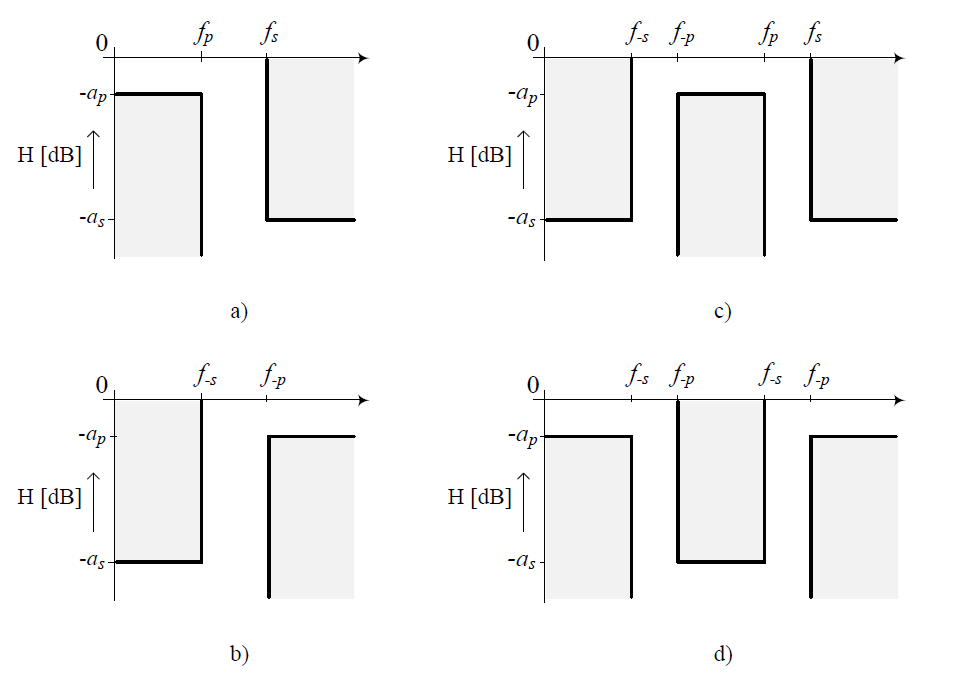
\includegraphics[scale=0.55]{tolerancnischemata.png}
\caption[Toleranční schéma]{Toleranční schéma pro a) dolní propust (DP), b) horní propust (HP), c) pásmovou propust (PP) a d) pásmovou zádrž (PZ)\cite{1}}
\end{figure}
\noindent Filtry se používají k redukci nežádoucích frekvencí např. pro efektivní reprodukci zvuku reproduktory, k redukci okolního rušení - vysílače blokují harmonické frekvence, které interferují. Také v obvodech rekonstrukce signálů u D/A převodníků, k předvzorkování u A/D převodníku nebo jako anti-aliasing filtry.\\\\
Obecná přenosová funkce filtru typu dolní propust je
\begin{equation}
H(j\omega) = \frac{H_0}{\prod_{i=1}^{\frac{n}{2}} (1 + a_i s + b_i s^2)},
\end{equation}
kde $n$ je řád filtru.\\
Obecná přenosová funkce filtru typu horní propust je
\begin{equation}
H(j\omega) = \frac{H_{\infty}}{\prod_{i=1}^{\frac{n}{2}} (1 + \frac{a_i}{s} + \frac{b_i}{s^2})},
\end{equation}
kde $n$ je řád filtru.\\
Podle rozložení nul a pólů jmenovatele rozlišujeme různé aproximace. Koeficienty filtru $a_i, b_i$ určují zesílení v propustném pásmu. Činitel jakosti je definován jako $Q = \sqrt{b_i}/a_i$. Čím větší $Q$ je obdrženo, tím spíš bude filtr nestabilní.
\begin{figure}[h]
\centering
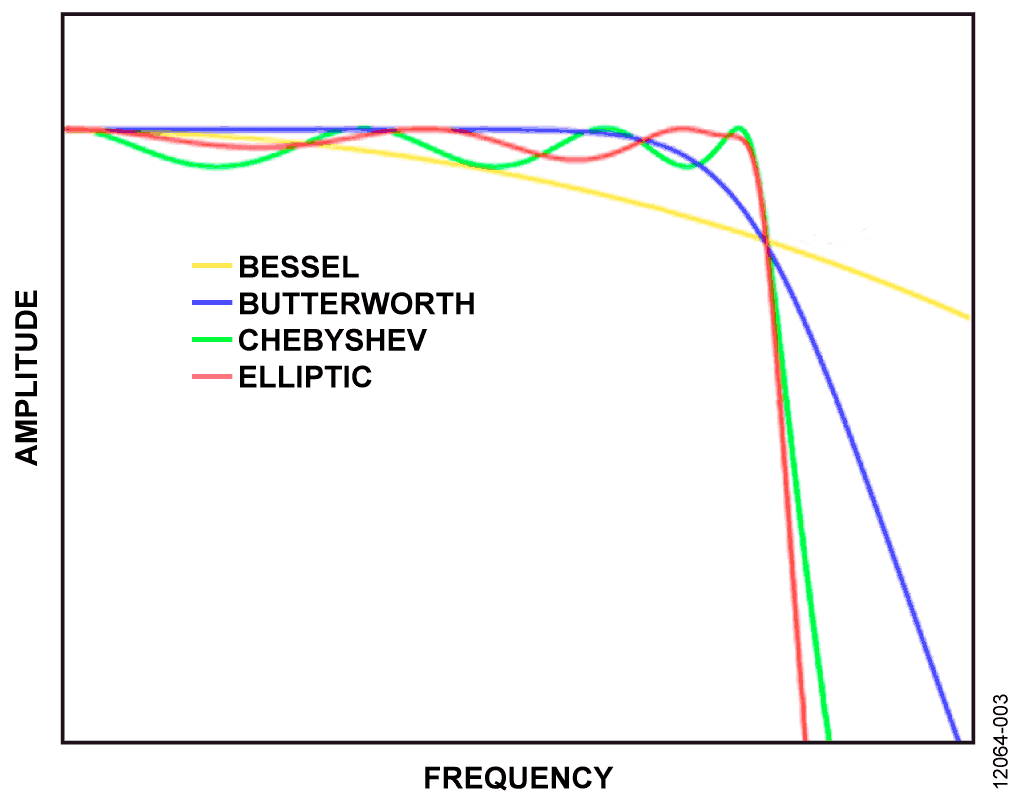
\includegraphics[scale=0.3]{LGA98.png}
\caption[Typy aproximací (DP)]{Typy aproximací (DP)\cite{2}}
\end{figure}
\subsection{Butterworthova aproximace}
Butterworthova má maximálně plochou amplitudovou charakteristiku v propustném pásmu. Frekvenční charakteristika má sklon daný počtem pólů a pro její posouzení je užíváno skupinové zpoždění (derivace fáze podle frekvence). Pro Butterworthovu aproximaci je skupinové zpoždění nezvlněné v propustném pásmu. Přechodová charakteristika má mírný překmit, zvyšující se s řádem filtru. Zesílení $G(\omega)$ je kmitočtově závislé a odpovídá absolutní hodnotě přenosové funkce $H(j\omega)$.
\begin{equation}
G(\omega) = |H(j\omega)| = \frac{1}{\sqrt{1 + \epsilon ^2 \frac{\omega}{\omega _c}^{2n}}},
\end{equation}
kde $\epsilon$ je poměrné zvlnění kmitočtové charakteristiky v propustném pásmu (\textit{faktor zvlnění}), $n$ je řád filtru a $\omega _c$ mezní kmitočet (nastává při útlumu -3 dB). Pro $\omega _c = 1$ je faktor zvlnění $\epsilon = 1$. 
\subsection{Čebyševova aproximace}
Čebyševova aproximace má strmější pokles, což vede k užití nižšího řádu filtru. Zato má ale zvlněnou frekvenční charakteristiku v propustném pásmu. 
\subsubsection{Typ I}
Vyjádření modulové charakteristiky pro tuto aproximaci je dáno jako
\begin{align}
G(\omega) = |H(j\omega)| = \frac{1}{\sqrt{1 + \epsilon ^2 T_n ^2 \frac{\omega}{\omega _c}^{2n}}},
\end{align}
kde $T_n$ je Čebyševův polynom, $\epsilon$ je poměrné zvlnění, $n$ je řád filtru a $\omega _c$ mezní kmitočet. Čebyševův polynom je definován vztahem $2 \omega ^2 - 1$ pro $n = 2$. Obecně jsou to kořeny Chebyshevových diferenciálních rovnic
\begin{align}
(1 - x^2)y" - xy' + n^2y &= 0\\
(1 - x^2)y" - 3xy' + n(n+2)y &= 0.
\end{align}
\subsubsection{Typ II}
Typ II je nazýván také jako inverzní Čebeševova aproximace. V praxi není příliš používaný, jelikož nemá tak rychlý pokles jako typ I a k jeho realizaci je třeba více prvků. Nemá zvlnění v propustném pásmu, zato v zádržném ano. Zesílení je definováno jako
\begin{equation}
G(\omega, \omega _c) = \frac{1}{\sqrt{1 + \frac{1}{\epsilon ^2 T_n ^2 \frac{\omega _c}{\omega}^{2n}}}},
\end{equation}
kde $T_n$ je Čebyševův polynom, $\epsilon$ je poměrné zvlnění, $n$ je řád filtru a $\omega _c$ mezní kmitočet.
\subsection{Besselova aproximace}
Besselova aproximace se používá v telekomunikační technice v případech, kdy je požadováno zachování tvaru signálu. Amplitudová charakteristika v nepropustném pásmu je velmi plochá. Koeficienty polynomu jsou zvoleny tak, aby fázová charakteristika v pásmu okolo kritické frekvence byla maximálně lineární. Nevýhodou je poměrně malá strmost modulové charakteristiky. Ta je pro Besselovu aproximaci dána vztahem
\begin{equation}
G(\omega) = |H(j\omega)| = \frac{\Theta _n(0)}{\Theta _n(\frac{j\omega}{\omega _c})},
\end{equation}
kde $\Phi _n$ je Besselův polynom a $\omega _c$ mezní kmitočet. Besselův polynom je definován součtem řady (Grosswald 1978, Berg 2000)
\begin{equation}
\Theta _n (x) = x^n y_n (\frac{1}{x}) = \sum_{k=0}^{n}\frac{(n+k)!}{(n-k)!k!}\frac{x^{n-k}}{2^k}.
\end{equation}
Pro filtr druhého řádu platí
\begin{equation}
G(\omega) = |H(j\omega)| = \frac{3}{\sqrt{\omega ^4 + 3\omega ^2 + 9}}.
\end{equation}
\subsection{Cauerova (eliptická) aproximace}
\noindent Cauerova aproximace (eliptická) má nejstrmější pokles, při jejím užití jsou voleny nižší řády filtru. Pokud se zvlnění v zádržném pásmu blíží nule, filtr se stává Čebyševovým (výše zmíněný - typ I). Opačně je tomu v propustném pásmu - přiblížením k nule se filtr stává inverzním Čebyševovým (typ II).  Pokud se obě hodnoty zvlnění blíží k nule, filtr se stává Butterworthovým. Kmitočtová charakteristika je dána vztahem
\begin{equation}
G(\omega) = |H(j\omega)| = \frac{1}{\sqrt{1 + \epsilon ^2 R_n ^2(\zeta, \frac{\omega}{\omega _c})}},
\end{equation}
kde $\epsilon$ je faktor zvlnění, $R_n$ eliptická racionální funkce n-tého řádu, $\zeta$ selektivní faktor a $\omega _c$ mezní kmitočet. Pokud pro selektivní faktor platí $\zeta \rightarrow \infty$, filtr se stává Čebyševovým (typ I).\\
Protože se, podobně jako u Čebyševovy aproximace, liší odvození pro liché a sudé stupně, jsou pro ně různé postupy. Pro lichý stupeň existuje pouze jedna varianta, pro sudý tři varianty (A, B, C), které se liší průběhem aproximační funkce.
\subsubsection{Cauerova (eliptická) aproximace typu A}
Má stejný počet pólů a nul aproximující funkce. Je realizována jako LC filtr (Sekce \ref{s:LC}) pouze s vázanými induktory.
\subsubsection{Cauerova (eliptická) aproximace typu B}
Jedná se o posun útlumového pólu z konečného kmitočtu k nekonečnu, tedy dále od propustného pásma. Tato úprava vede ke snížení strmosti přechodu od propustného k nepropustnému pásmu. Je to obdoba postupu u inverzní Čebyševovy aproximace.
\subsubsection{Cauerova (eliptická) aproximace typu C}
Vhodnou transformací, která vede na nulovou hodnotu přenosu v nulovém kmitočtu, získáme navíc proti variantám A, B i shodné zakončovací odpory v případě LC realizace (Sekce \ref{s:LC}). Je to obdoba postupu u Čebyševovy aproximace.
\subsection{Srovnání typů aproximací}
Z hlediska zápisu přenosové funkce není rozdíl mezi Butterworthovou a Čebyševovou aproximací, přestože jedna má v propustném pásmu hladký a druhá zvlněný průběh. Přenosová funkce má v čitateli konstantu a ve jmenovateli polynom (odtud společné označení polynomiální aproximace).\\
Oproti tomu volba průběhu v nepropustném pásmu tvar přenosové funkce mění. Pokud je průběh monotónní (Butterworthova, Čebyševova aproximace), jedná se o podíl konstanty a polynomu. Je-li průběh v nepropustném pásmu zvlněný, tvoří přenosovou funkci podíl dvou polynomů. Pro běžné aproximace (Cauerova, inverzní Čebyševova) je v čitateli sudý polynom ve tvaru $\prod _{i} (p^2 + \omega_i^2)$.\\
Volbou kombinace hladkého a zvlěného průběhu v propustném a nepropustném pásmu získáme různé vlastnosti.\\
 \begin{table}[h]
 \caption[Přehled aproximací podle tvaru aproximační funkce v propustném i nepropustném pásmu]{\label{tab:Přehled aproximací podle tvaru aproximační funkce v propustném i nepropustném pásmu}Přehled aproximací podle tvaru aproximační funkce v propustném i nepropustném pásmu \cite{3}}
  \end{table}
\begin{center}
\begin{table}[h]
\centering
  \begin{tabular}{ | c | c | c | }
    \hline
    Propustné pásmo & Nepropustné pásmo & Příklad aproximace \\ \hline
    hladká & hladká & Butterworthova \\ \hline
    zvlněná & hladká & Čebyševova \\ \hline
    hladká & zvlněná & inverzní Čebyševova \\ \hline
    zvlněná & zvlněná & Cauerova \\ \hline
  \end{tabular}
   \end{table}
   \end{center}
\sekce{Transkonduktanční zesilovače (OTA)}
V telekomunikacích se používají filtry v rozsahu kmitočtů desítek až stovek megahertz, v bezdrátové komunikaci až v řádu gigahertz. Běžné RC filtry by neměly být užívány ve frekvenčním rozsahu nad 5--10 $\%$ $\omega _c$ - tedy v tomto rozsahu používaném v telekomunikačních technologiích nemají předvídatelné průběhy. Krom toho ve spínačích CMOS, kde rezistory běžně nejsou dostupné, jsou potřeba zesilovače s velkou šířkou pásma a zároveň vysokým zesílením. Dodržení těchto požadavků je náročné a drahé. Dalším extrémem pro analogové integrované filtry jsou telefonní linky, kde jsou kmitočtové rozsahy sice nízké, ale je požadována nízká cena a vysoká přesnost.\\
\\
Pro nízké frekvence se ke splnění těchto požadavků používají obvody se spínanými kapacitory (SC). Přepínaný kapacitor se chová jako rezistor, tudíž časová konstanta RC je definována poměrem kapacitorů a hodinovou (CLK) frekvencí, se kterou jsou přepínány. Pro vysokofrekvenční aplikace (až v řádu gigahertz) se používají MOSFET-C filtry.\\
\\
Další z možných prvků, které jsou dostupné jak pro nízkofrekvenční aplikace, tak pro kmitočtový rozsah stovek megahertz, jsou transkonduktanční zesilovače.\\
\\
Transkonduktanční zesilovače (označují se též jako OTA (\textit{Operational Transconductance Amplifiers}) jsou napětím řízené zesilovače s proudovým výstupem - zdroje proudu
\begin{equation}
i_{out} = g_m(u_+ - u_-),
\end{equation}
kde $u_+$ a $u_-$ jsou napětí invertujícího a neinvertujícího vstupu.  Transkonduktance je řízena externím proudem $I_{ABC}$ (\textit{Bias Current}). Ideální OTA má kmitočtově nezávislou transkonduktanci $g_m$ (na rozdíl od reálného, který je kmitočtově závislý).
\begin{figure}[h]
\centering
\includegraphics[scale=0.7]{image7.png}
\caption[OTA - schematické značky]{OTA - schematické značky \cite{4}}
\end{figure}
\begin{figure}[h]
\centering
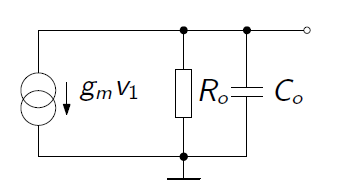
\includegraphics[scale=0.6]{gmrc.png}
\caption[Linearizovaný model reálného OTA]{Linearizovaný model reálného OTA \cite{5}}
\end{figure}
\noindent Připojením zátěže $R_z$ na výstup bylo získáno napětí naprázdno
\begin{equation}\label{s:vzt}
u_{out} = R_zg_m(u_+ - u_-) = G_0(u_+ - u_-),
\end{equation}
kde $G_0$ je zesílení. Ze vztahu \ref{s:vzt} plyne, že zesílení je konečné a mezi vstupy je nenulové napětí. Připojením kondenzátoru jako zátěže byl získán bezeztrátový integrátor s přenosem
\begin{equation}
H(s) = \frac{v_2}{v_1} = \frac{g_m}{sC}
\end{equation}
\noindent a napětím na výstupu
\begin{equation}
v_0(t) = \frac{1}{C}\int i(t)dt = \frac{1}{C}\int g_mv_1(t)dt.
\end{equation}
\begin{figure}[h]
\centering
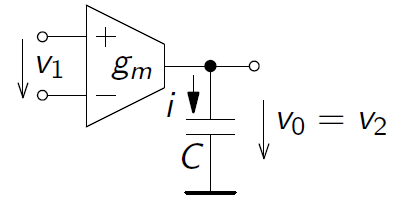
\includegraphics[scale=0.5]{otaintegrator.png}
\caption[OTA-C]{OTA-C \cite{5}}
\end{figure}
\noindent Toto zapojení integrátoru s uzemněným kondenzátorem se označuje jako OTA-C.\\
\\
Ztrátový integrátor lze utvořit sériovým zapojením dalšího OTA jako odporu se zápornou zpětnou vazbou. Rozdíl mezi ideálním a ztrátovým integrátorem lze pozorovat i v modulové charakteristice - pro ztrátový je konstantní a pak teprve lineárně klesá se sklonem -20 dB/dek.
\begin{equation}
v_0(t) = \frac{g_{m1}}{sC + g_{m2}}(v_1^+ - v_{1}^-)
\end{equation}
\begin{figure}[h]
\centering
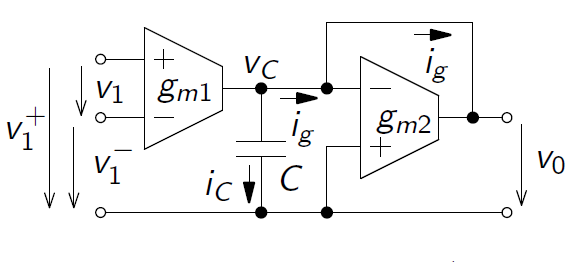
\includegraphics[scale=0.5]{damp.png}
\caption[Ztrátový OTA-C]{Ztrátový OTA-C \cite{5}}
\end{figure}
\subsection{Current Conveyor of Second Generation (CCII) s OTA}
Jeden z nejzákladnějších bloků v oblasti analogov obvodů v proudovém módu je \textit{current conveyor (CC)}. Princip CC první generace byl popsán v roce 1968 (K. C. Smith, A. S. Sedra \cite{6}). \textit{CCI} byl následně nahrazen univerzálnější druhou generací v roce 1970 (\textit{CCII})\cite{7}. Obvody s CC se používaly především v zapojeních s bipolárními tranzistory kvůli jejich vysoké transkonduktanci (v porovnání s CMOS). Jsou to operační zesilovače s proudovou zpětnou vazbou (např. MAX477, MAX4112). \textit{Current conveyors} jsou používány ve vysokofrekvenčních obvodech, kde je problematické použití běžných operačních zesilovačů, protože jsou limitovány násobkem šířky pásma a zesílení (\textit{gain-bandwidth product}). Je to struktura s třemi vstupy.
\begin{figure}[h]
\centering
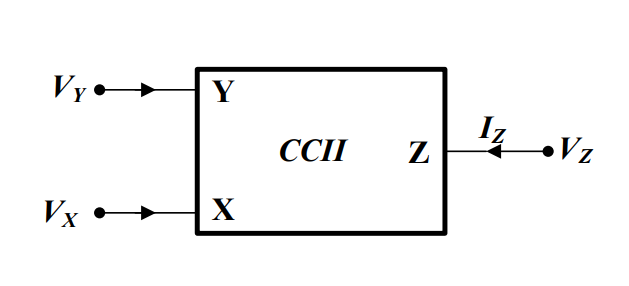
\includegraphics[scale=0.4]{ccii.png}
\caption[CCII symbol]{CCII symbol \cite{8}}
\end{figure}
\noindent Vstupní impedance na vstupu Y je nekonečná (tedy proud tekoucí skrz Y je nulový) a impedance na vstupu X je nulová ($R_Y = \infty, I_Y = 0, R_X = 0$). Napětí na vstupu X je ekvivalentní k napětí na vstupu Y ($V_X = V_Y$). Proud procházející vstupem X je ekvivalentní k proudu vstupem Z ($I_Z = I_X$). Výstupní impedance vstupu Z je nekonečná ($R_Z = \infty$).
Charakteristika ideálního \textit{CC} je reprezentována maticí
\begin{equation}
\begin{bmatrix}
I_Y \\ V_X \\ I_Z
\end{bmatrix}
=
\begin{bmatrix}
0 & 0 & 0 \\
1 & 0 & 0 \\
0 & \pm 1 & 0 
\end{bmatrix}
\begin{bmatrix}
V_Y \\
I_X \\
V_Z
\end{bmatrix}.
\end{equation}
\begin{figure}[h]
\centering
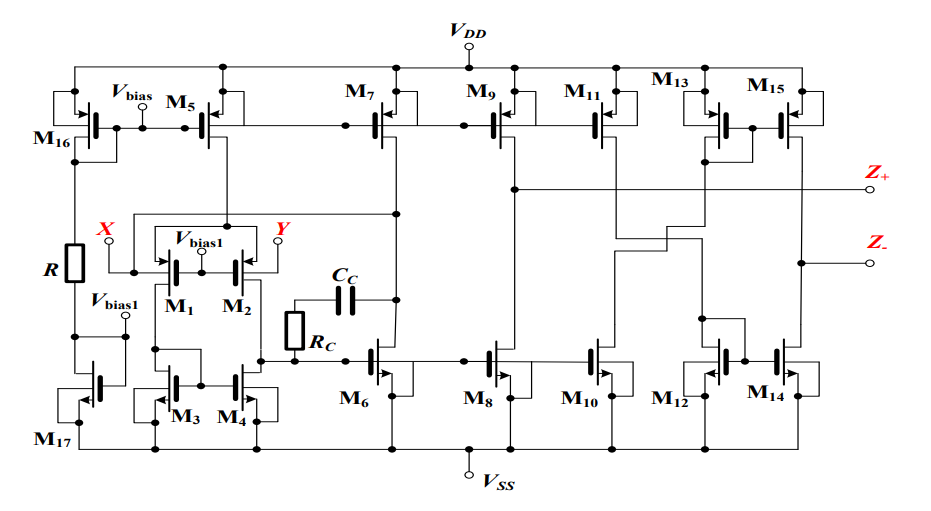
\includegraphics[scale=0.45]{cciiota.png}
\caption[CCII s $\pm$ výstupem založený na OTA]{CCII s $\pm$ výstupem založený na OTA \cite{8}}
\end{figure}
\noindent Takovéto zapojení funguje jako dobrý sledovač napětí, ale zato má menší šířku pásma.\\
\newline
Využitím zapojení na obrázku \ref{s:OTA} a principů \textit{CCII} lze získat modifikace klasického transkonduktančního zesilovače (s rozdílovým stupněm na vstupu a jedním výstupem). Obdržené atypické struktury obsahují jeden vstup a jeden výstup a také dva rozdílové stupně (na vstupu i výstupu).
\begin{figure}[h]
\centering
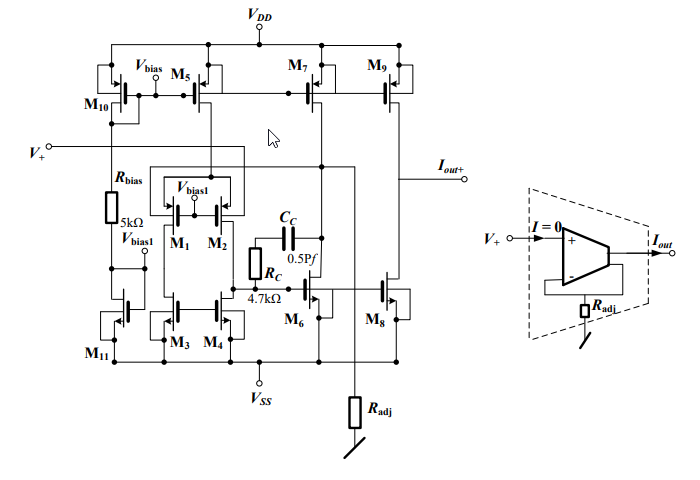
\includegraphics[scale=0.6]{siso.png}
\caption[Single input single output OTA (SISO) založený na CCII]{Single input single output OTA (SISO) založený na CCII \cite{8}}
\end{figure}
\begin{figure}[h]
\centering
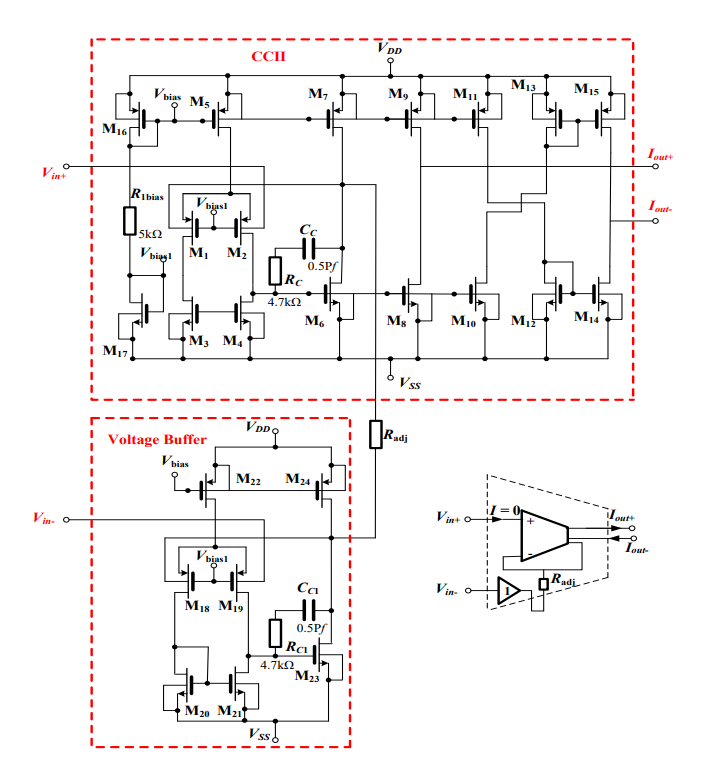
\includegraphics[scale=0.6]{dido.png}
\caption[\textit{Fully differential} OTA (DIDO) založený na CCII a napěťovém bufferu]{\textit{Fully differential} OTA (DIDO) založený na CCII a napěťovém bufferu \cite{8}}
\end{figure}
\newpage
\subsection{Integrované obvody s OTA}
Integrované obvody se vyrábí buď s jedním nebo dvěma zesilovači v pouzdře. Varianty s jedním operačním zesilovačem jsou např. OPA615, OPA860 a novější OPA861. Všechny součástky s jedním OTA mají velkou šířku pásma (v řádech stovek MHz), cenově vychází na 75--280 Kč. Integrované obvody s dvěma zesilovači v pouzdře mají užší šířku pásma (2 MHz), menší rychlost přeběhu (50 V/$\mu$s), mnohem menší výstupní proud (650 $\mu$A) i offset vstupního napětí a operují při cca 4x nižších proudech. Cenové rozpětí je 25--65 Kč.
\renewcommand{\arraystretch}{1.5}
\begin{table}[h]
\scalebox{0.9}{%
  \begin{tabular}{ | c | >{\centering\arraybackslash}p{2cm}| >{\centering\arraybackslash}p{1.5cm} | >{\centering\arraybackslash}p{1.5cm} | >{\centering\arraybackslash}p{1.25cm} | >{\centering\arraybackslash}p{1.5cm} | >{\centering\arraybackslash}p{1.75cm} | >{\centering\arraybackslash}p{2cm} | >{\centering\arraybackslash}p{1.75cm} |}
    \hline
      & GBP - Gain Bandwidth Product & SR - Slew Rate & Output Current per Channel & $I_b$ - Input Bias Current & $V_{os}$ - Input Offset Voltage & Operating Supply Current & Forward Transconductance Min & Supply Voltage\\ \hline
    OPA615 & 710 MHz & 2.5 kV/$\mu$s & 5 mA & 3 $\mu$A & 40 mV & 13 mA & 65 mA/V & 8--12.4 V \\ \hline
    OPA860 & 470 MHz & 3.5 kV/$\mu$s & 15 mA & 5 $\mu$A & 12 mV & 11.2 mA & 80 mA/V & 5--13 V \\ \hline
    OPA861 & 400 MHz & 900 V/$\mu$s & 15 mA & 1 $\mu$A & 12 mV & 5.4 mA & 65 mA/V & 4--12.6 V  \\
    \hline
  \end{tabular}}
  \caption[Porovnání integrovaných obvodů s jedním OTA]{\label{tab:Porovnání integrovaných obvodů s jedním OTA}Porovnání integrovaných obvodů s jedním OTA \cite{9}}
  \end{table}
\begin{center}
\begin{table}[h]
\scalebox{0.9}{%
  \begin{tabular}{ | c | >{\centering\arraybackslash}p{2cm}| >{\centering\arraybackslash}p{1.5cm} | >{\centering\arraybackslash}p{1.5cm} | >{\centering\arraybackslash}p{1.25cm} | >{\centering\arraybackslash}p{1.5cm} | >{\centering\arraybackslash}p{1.75cm} | >{\centering\arraybackslash}p{2cm} | >{\centering\arraybackslash}p{1.75cm} |}
    \hline
      & GBP - Gain Bandwidth Product & SR  - Slew Rate & Output Current per Channel & $I_b$ - Input Bias Current & $V_{os}$ - Input Offset Voltage & Operating Supply Current & Forward Transconductance - Min & Supply Voltage\\ \hline
    LM13700 & 2 MHz & 50 V/$\mu$s & 650 $\mu$A & 5 $\mu$A & 4 mV & 1.3 mA & 6700 $\mu$S & 10--36 V \\ \hline
    NE5517 & 2 MHz & 50 V/$\mu$s & 650 $\mu$A & 5 $\mu$A & 5 mV & 2.6 mA & 5400 $\mu$S & 4--44 V \\ \hline
    AU5517 & 2 MHz & 50 V/$\mu$s & 650 $\mu$A & 5 $\mu$A & 5 mV & 2.6 mA & 5400 $\mu$S & 4--44 V  \\ \hline
    NJM13600 & 2 MHz & 50 V/$\mu$s & 650 $\mu$A & 5 $\mu$A & 5 mV & 2.6 mA & 6700 $\mu$S & 36 V  \\ \hline
    NJM13700 & 2 MHz & 50 V/$\mu$s & 650 $\mu$A & 5 $\mu$A & 4 mV & 2.6 mA & 6700 $\mu$S & 36 V  \\ \hline
  \end{tabular}}
  \caption[Porovnání integrovaných obvodů se dvěma OTA]{\label{tab:Porovnání integrovaných obvodů se dvěma OTA}Porovnání integrovaných obvodů se dvěma OTA \cite{9}}
  \end{table}
\end{center}
\noindent Pro realizaci přeladitelného filtru byl zvolen LM13700.
\begin{figure}[h]
\centering
\includegraphics[scale=0.55]{image6.png}
\caption[Konfigurace pinů na LM13700M]{Konfigurace pinů na LM13700M \cite{10}}
\end{figure}
\noindent Vnitřní zapojení LM13700 na obrázku \ref{s:OTA} obsahuje symetrický rozdílový stupeň (tranzistory Q4, Q5), který je napájen řízeným zdrojem proudu s tranzistorem Q2. Dvojice diod a tranzistorů tvoří proudová zrcadla (\textit{Current Mirror}) - referenční proud tekoucí v jedné větvi obvodu se \uv{zrcadlí} ~v jeho druhé větvi. Principiálně jsou to zdroje proudu řízené proudem. 
\begin{figure}[h]
\centering
\includegraphics[scale=0.75]{image5.png}
\caption[Vnitřní schéma OTA]{Vnitřní schéma OTA \cite{10}\label{sec:OTA}}
\end{figure}\label{s:OTA}
\sekce{Náhrada prvků}\label{s:NAH}
\noindent Podle literatury \cite{19} je pro ideální OTA zesilovač (vstupní i výstupní impedance nulové) možno odpor nahradit obvodem s uzemněným neinvertujícím vstupem a zpětnou vazbou z invertujícího vstupu na výstup a to hodnotou
\begin{align}
R_{in} = \frac{1}{g_{m}},
\end{align}
kde $g_{m}$ označuje transkonduktanci zesilovače. Prohození invertujícího a neinvertujícího vstupu vede na opačnou polaritu. Tato konfigurace jako odpor je užitečná např. k návrhu monolitických $g_m$-RC filtrů pouze s transkonduktancemi a kapacitami ($g_m$-C filtry - viz \ref{s:OTA}, \ref{s:GM-C}), také k náhradě velmi velkých odporů.
\begin{figure}[h]
\centering
\includegraphics[scale=0.45]{image10.png}
\caption[Náhradní obvod pro uzemněný rezistor]{Náhradní obvod pro uzemněný rezistor \cite{18}}
\end{figure}
\noindent Dále lze dle literatury \cite{18} pro nahrazení indukčnosti o impedanci $Z_L = 1/(sC)$ použít obvod s třemi OTA. Uzemněny jsou invertující vstup prvního OTA a neinvertující druhého. Použita je zpětná vazba z výstupu na neinvertující vstup prvního OTA. Propojení výstupu prvního OTA na invertující vstup druhého OTA je realizován přes uzemněný kapacitor. \\
Vyjádřením napětí a proudů v obvodu bylo získáno napětí na kapacitoru a vstupní proud
\begin{align}\label{s:vzt2}
V_C &= \frac{g_{m1}}{sC}V_1 \\
I_1 &= g_{m2}V_C = \frac{g_{m1}g_{m2}}{sC}V_1.
\end{align}
Výsledná indukčnost - impedance vstupu byla vyjádřena vztahem \ref{s:vzt2}.
\begin{align}
Z_{in}(s) = \frac{V_1}{I_1} = s\frac{C}{g_{m1}g_{m2}}
\end{align}
\noindent Byl obdržen induktor o hodnotě
\begin{align}
L = \frac{C}{g_{m1}g_{m2}}.
\end{align}
\begin{figure}[h]
\centering
\includegraphics[scale=0.45]{image13.png}
\caption[Náhradní obvod pro indukčnost]{Náhradní obvod pro indukčnost \cite{18} \label{s:IND}}
\end{figure}
\noindent Pro uzemněnou indukčnosti o impedanci $Z_L = 1/(sC)$ byl podle literatury \cite{18} použit obvod na obrázku \ref{s:IND}. Vyjádřením napětí a proudů v obvodu bylo získáno napětí na kapacitoru a vstupní proud
\begin{align}
V_C &= \frac{g_{m1}}{sC}V_1 \\
I_1 &= g_{m2}V_C = \frac{g_{m1}g_{m2}}{sC}V_1.
\end{align}
Výsledná indukčnost - impedance vstupu byla vyjádřena vztahem
\begin{align}
Z_{in}(s) = \frac{V_1}{I_1} = s\frac{C}{g_{m1}g_{m2}}.
\end{align}
\begin{figure}[h]
\centering
\includegraphics[scale=0.45]{image12.png}
\caption[Náhradní obvod pro neuzemněnou indukčnost]{Náhradní obvod pro neuzemněnou indukčnost pro $g_{m1} = g_{m2}$\cite{18}}
\end{figure}
\subsection{Základní bloky}
\begin{figure}[h]
\centering
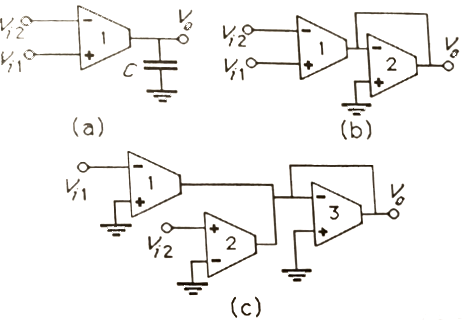
\includegraphics[scale=0.45]{otos.png}
\caption[Základní bloky s OTA]{Základní bloky s OTA a) integrující b) škálující c) sčítací \cite{18} \label{s:BLO}}
\end{figure}
\noindent Podle lieratury \cite{18} blok a) na obrázku \ref{s:BLO} slouží k realizaci invertujícího/neinvertujícího integrátoru s výsledným napětím
\begin{equation}
V_O = \frac{g_{m1}}{pC}(V_1 - V_2).
\end{equation}
Blok b) na obrázku \ref{s:BLO} je komparátor s různou polaritou a napětím na výstupu
\begin{equation}
V_O = \frac{g_{m1}}{g_{m2}}(V_1 - V_2).
\end{equation}
Blok c) na obrázku \ref{s:BLO} realizuje sčítací nebo rozdílový obvod s napětím na výstupu
\begin{equation}
V_O = -\frac{g_{m1}}{g_{m3}}V_1 + \frac{g_{m2}}{g_{m3}}V_2.\label{s:BLO3}
\end{equation}
\noindent Spojením těchto základních stavebních bloků se správnými znaménky lze získat různé funkční bloky.\\
Základním principem uplatňovaným při návrhu s OTA je použití pouze OTA a uzemněných kapacitorů, protože při návrhu IC (\textit{Integrated Circuit}) jsou uzemněné kapacitory méně zatíženy parazitními chybami než neuzemněné kapacitory. Pro IC použití je vhodné volit shodné transkonduktance. Parazitní vstupní a především výstupní impedance způsobují chyby ve výstupu filtru, což může vést na parazitní póly, které při vysokofrekvenčním použití nelze zanedbat. Při použití filtru pro zvukové aplikace (20 -- 20 000 Hz) lze chyby způsobené parazitními součástkami zanedbat, rovněž lze zanedbat chyby způsobené konečnou šířkou pásma.
\subsection{Odvození DP 2. řádu}\label{s:ODV}
\noindent Náhradní obvod, ze kterého bude spočítána přenosová funkce pro přenos filtru druhého řádu, popisuje obrázek \ref{s:DPO}.
\begin{figure}[h]
\centering
\includegraphics[scale=0.4]{circuit(2).png}
\caption{Dolní propust 2. řádu \label{s:DPO}} 
\end{figure}
\noindent Přenos obvodu byl vyjádřen jako
\begin{align}
H(s) = \frac{U_{out}}{U_{in}} = \frac{Z_2}{Z_1}, \quad Z_1 = sL,\quad Z_2 = \frac{\frac{R}{pC}}{R + \frac{1}{pC}}.
\end{align}
Výsledný přenos je roven 
\begin{align}
H(s) = \frac{\frac{\frac{R}{pC}}{R + \frac{1}{pC}}}{pL + \frac{\frac{R}{pC}}{R + \frac{1}{pC}}}.
\end{align}
Elementárními algebraickými úpravami a následným vynásobením členem $1/(LRC)$ byl získán výsledný přenos.
\begin{align}\label{s:vzt4}
H(s) = \frac{R}{p^2LRC + sL + R} = \frac{\frac{1}{LC}}{p^2 + \frac{p}{RC} + \frac{1}{LC}}.
\end{align}
\noindent Využitím poznatků ze Sekce \ref{s:NAH} je možno za odpor a indukčnost dosadit do vztahu \ref{s:vzt4}. Byly uvažovány kapacitory o stejné hodnotě C.
\begin{align}
H(s) = \frac{\frac{1}{\frac{C^2}{g_{m1}g_{m2}}}}{p^2 + \frac{p}{\frac{C}{g_{m2}}} + \frac{1}{\frac{C^2}{g_{m1}g_{m2}}}} = \frac{\frac{g_{m1}g_{m2}}{C^2}}{p^2 + \frac{pg_{m2}}{C} + \frac{g_{m1}g_{m2}}{C^2}} = \frac{g_{m1}g_{m2}}{p^2C^2 + pg_{m2}C + g_{m1}g_{m2}}.
\end{align}
Porovnáním jmenovatele se jmenovatelem přenosu filtru 2. řádu byl obdržen vztah
\begin{align}
p^2 + p\frac{\omega _c}{Q} + \omega _c^2 &= p^2C^2 + pg_{m2}C + g_{m1}g_{m2}\\
p^2 + p\frac{\omega _c}{Q} + \omega _c^2 &= p^2 + \frac{pg_{m2}}{C} + \frac{g_{m1}g_{m2}}{C^2}.
\end{align}
Z tohoto vztahu byl vyjádřen mezní kmitočet jako 
\begin{align}
\omega _c^2 &= \frac{g_{m1}g_{m2}}{C^2} \\
\omega _c &= \sqrt{\frac{g_{m1}g_{m2}}{C^2}}
\end{align}
a činitel jakosti dosazením za $\omega _c$
\begin{align}
Q = \frac{\omega _c}{\frac{g_{m2}}{C}} = \sqrt{\frac{g_{m1}}{g_{m2}}}.
\end{align}
Pokud navíc byly uvažovány stejné transkonduktance $g_{m1}, \ g_{m2} = g_m$, byl obdržen výsledek
\begin{align}
\omega _c &= \sqrt{\frac{g_m^2}{C^2}},\\
Q &= \sqrt{1} = 1.
\end{align}
\sekce{Simulace}
\subsection{Dolní propust 2. řádu}\label{s:DP2}
Dolní propust druhého řádu má přenos v nekonečnu nulový $H_{\infty} = 0$. Přenosová funkce je
\begin{align}
H(j\omega) = \frac{H_0 \omega_c ^2}{(j\omega)^2 + \frac{\omega _c}{Q}(j\omega) + \omega _c ^2}.
\end{align}
\noindent Obvodová simulace byla realizována v programu Multisim. Bylo zvoleno symetrické napájení OZ $V_{DD},V_{SS} = \pm 15$ V. Regulací vstupního proudu je ovlivňován pracovní bod obvodu (mezní kmitočet). Vstupní externí proud $I_{ABC} = 0.5$ $\mu$A byl zvolen tak, aby byl obdržen mezní kmitočet cca 100 kHz. Externím proudem $I_{ABC} \in$ $[5$ $\mu$A ; 500 $\mu$A] je garantováno minimální výstupní napětí $U_{OUT} = \pm 12$ V, standardně $V_{peak 1} = 14.2$ V a $V_{peak 2} = -14.4$ V. Při výstupním napětí v tomto intervalu je šum vzhledem k signálu zanedbatelný a nezkreslí výsledky simulace.\\
\noindent Bylo použito zapojení s paralelně řazeným uzemněným kapacitorem a odporem a indukčností. Na výstupu 2. OTA (V1) byl obdržen filtr typu PP 1. řádu. Na výstupu 3. OTA (V2) pak DP 2. řádu.
\begin{figure}[H]
\centering
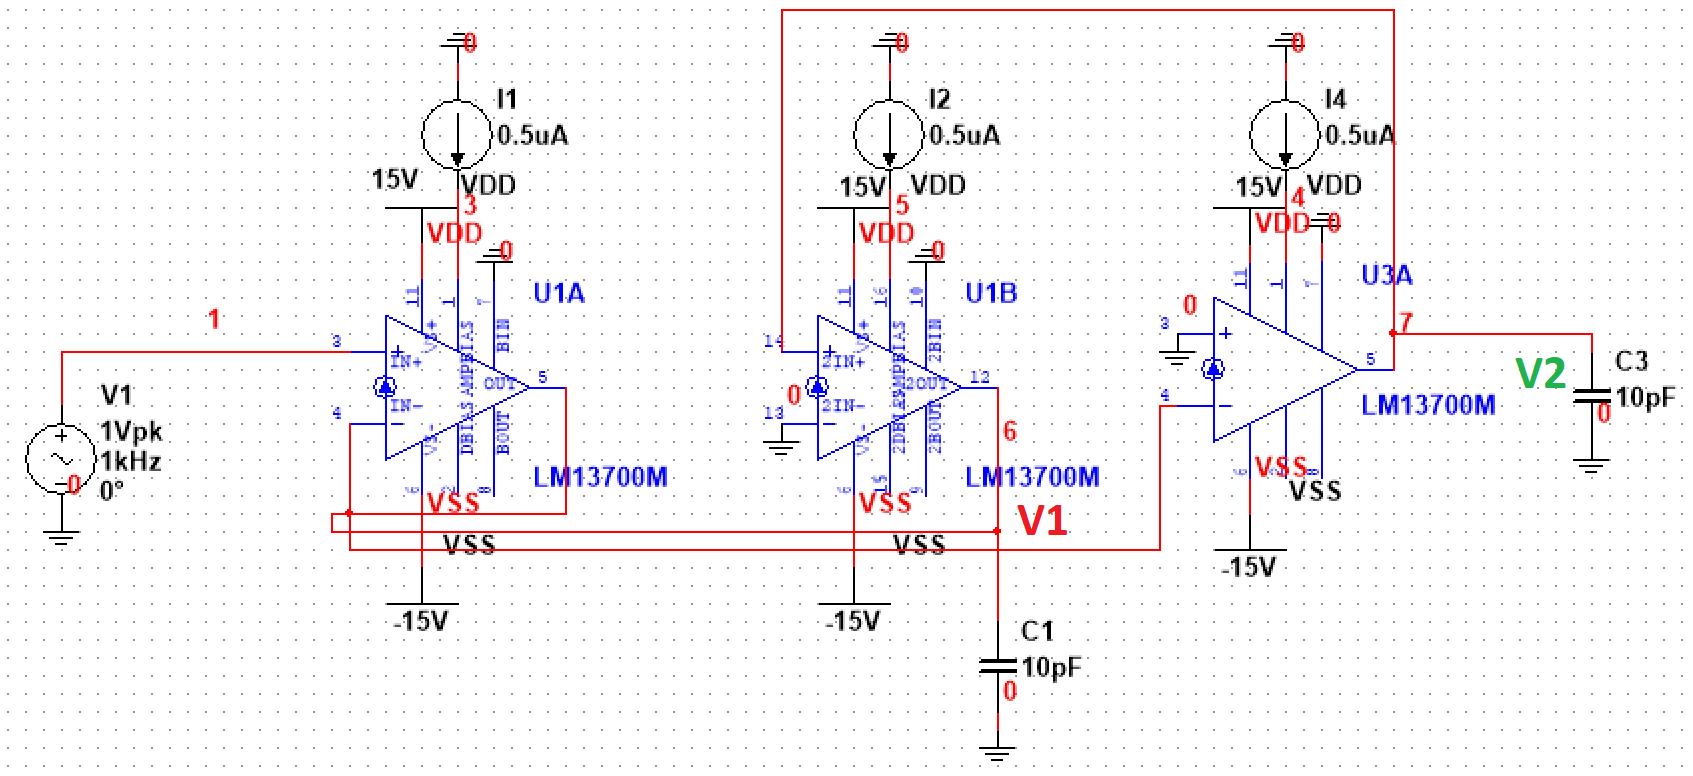
\includegraphics[scale=0.3]{bplp.png}
\caption{Schéma zapojení DP 2. řádu}
\end{figure}\begin{figure}[H]
\centering
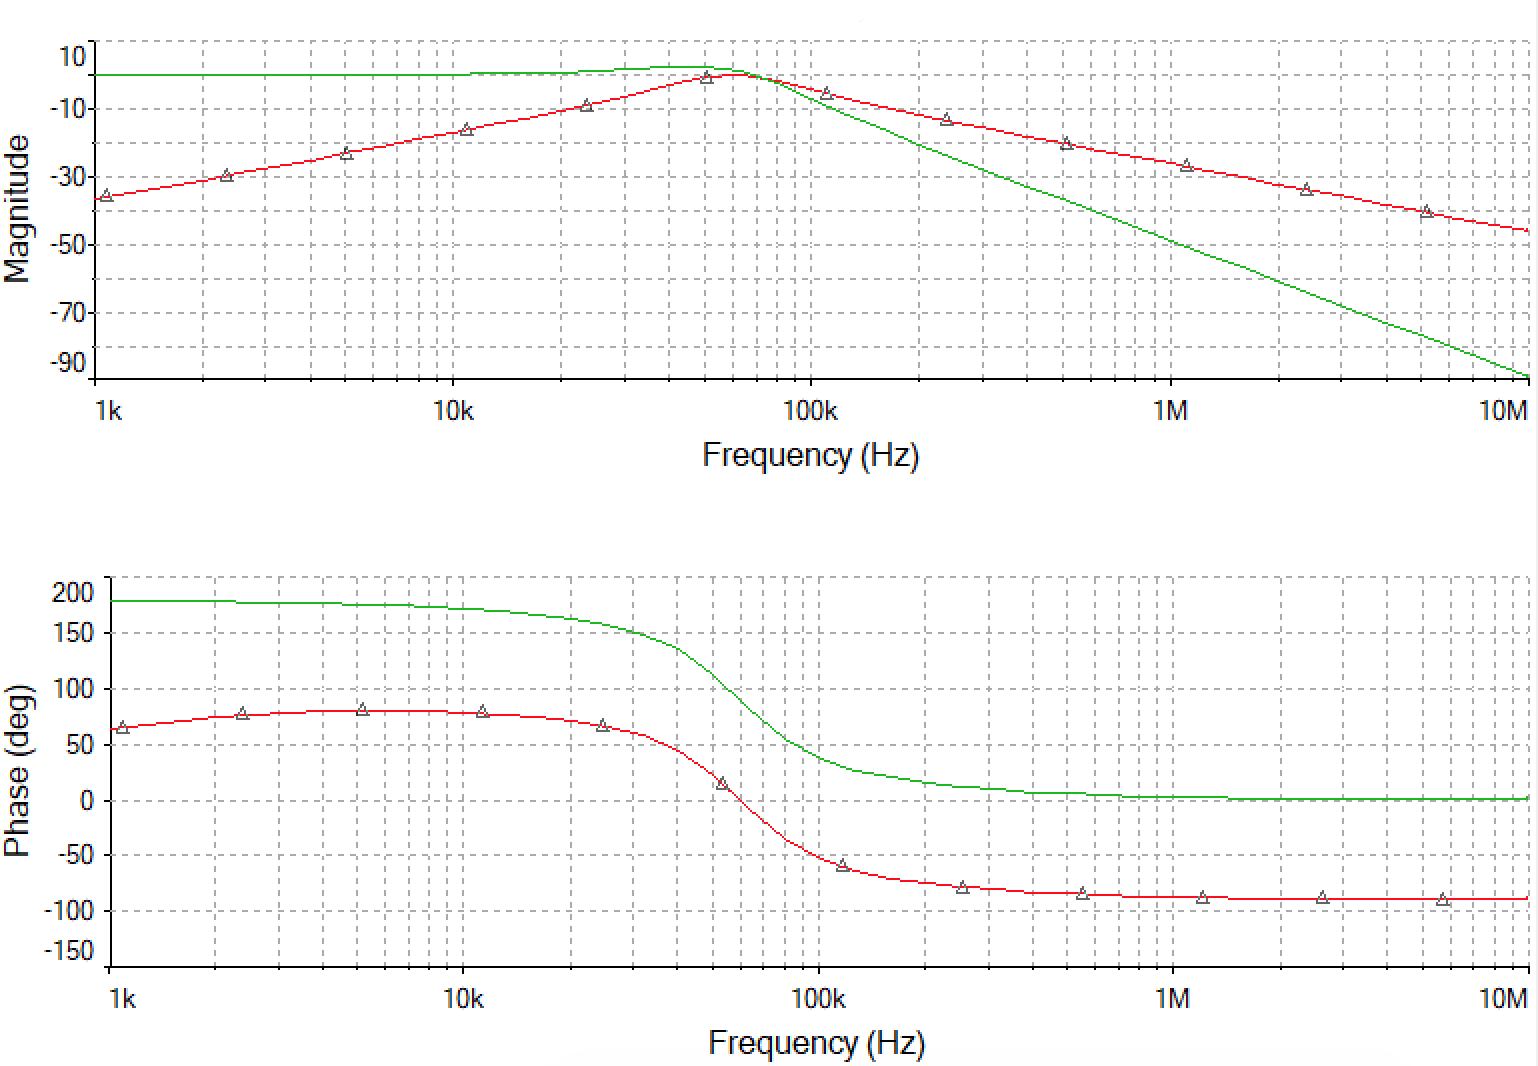
\includegraphics[scale=0.5]{bplp2.png}
\caption{Amplitudová a fázová charakteristika DP 2. řádu, PP}
\end{figure}
\subsection{Dolní propust 4. řádu}\label{s:DP4}
Kaskádní zapojení sestává ze sériově zapojených bloků.
\begin{figure}[H]
\centering
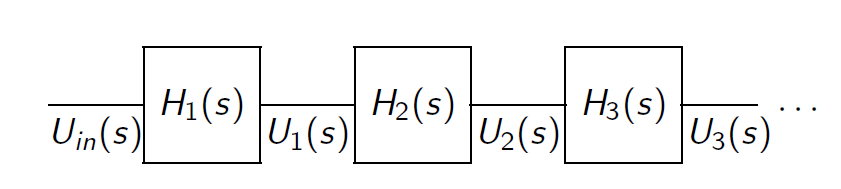
\includegraphics[scale=0.4]{schemata.png}
\caption{Kaskádní zapojení \cite{5}}
\end{figure}
\noindent Přenosové funkce jednotlivých bloků se násobí
\begin{align}
H_k(j\omega) = \frac{U_k (j\omega)}{U_{k-1}(j\omega)}.
\end{align}
Přenos posledního bloku je dán vztahem
\begin{align}
H_{1 \rightarrow k}(j\omega) = \frac{U_k (j\omega)}{U_{in}(j\omega)} = \prod _{n=1}^{k} H_n(j\omega).
\end{align}
Kaskádním zapojením dvou dolních propusti ze sekce \ref{s:DP2} byl obdržen filtr 4. řádu s poklesem -80 dB/dek.
\begin{figure}[H]
\centering
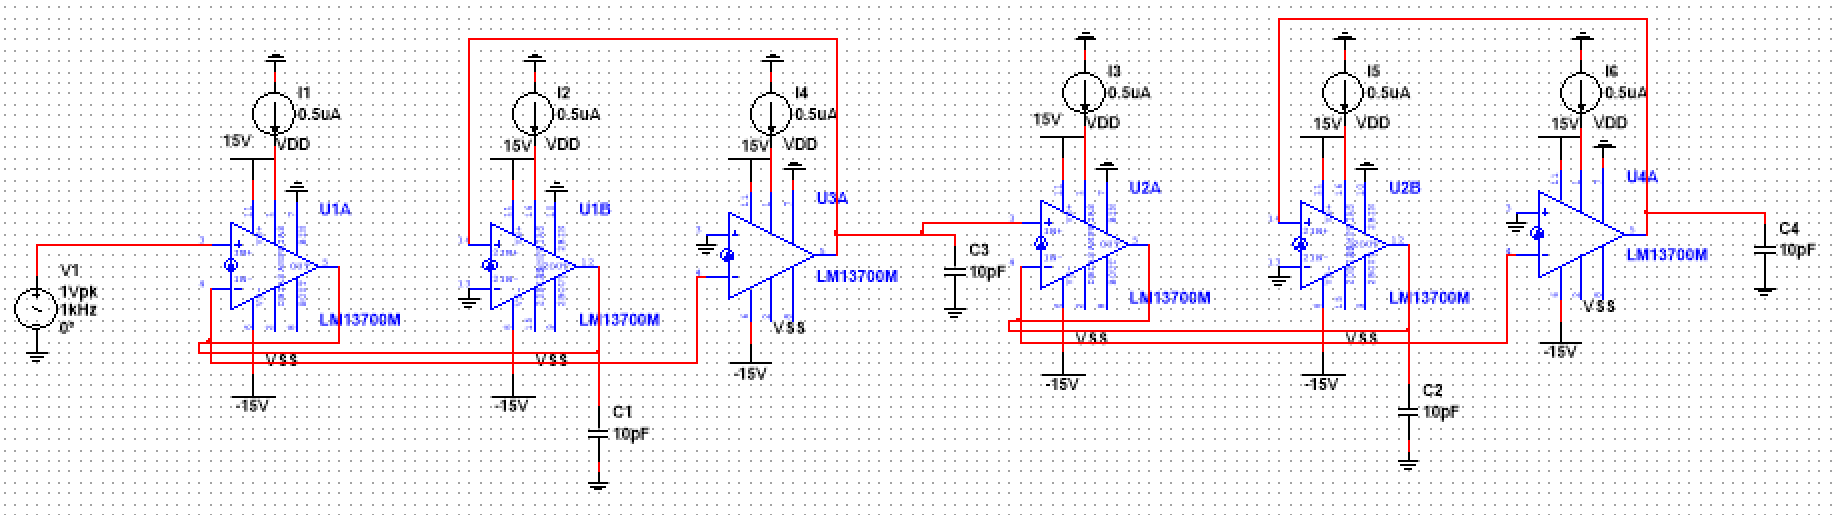
\includegraphics[scale=0.5]{lpbp32.png}
\caption{Schéma zapojení DP 4. řádu}
\end{figure}\begin{figure}[H]
\centering
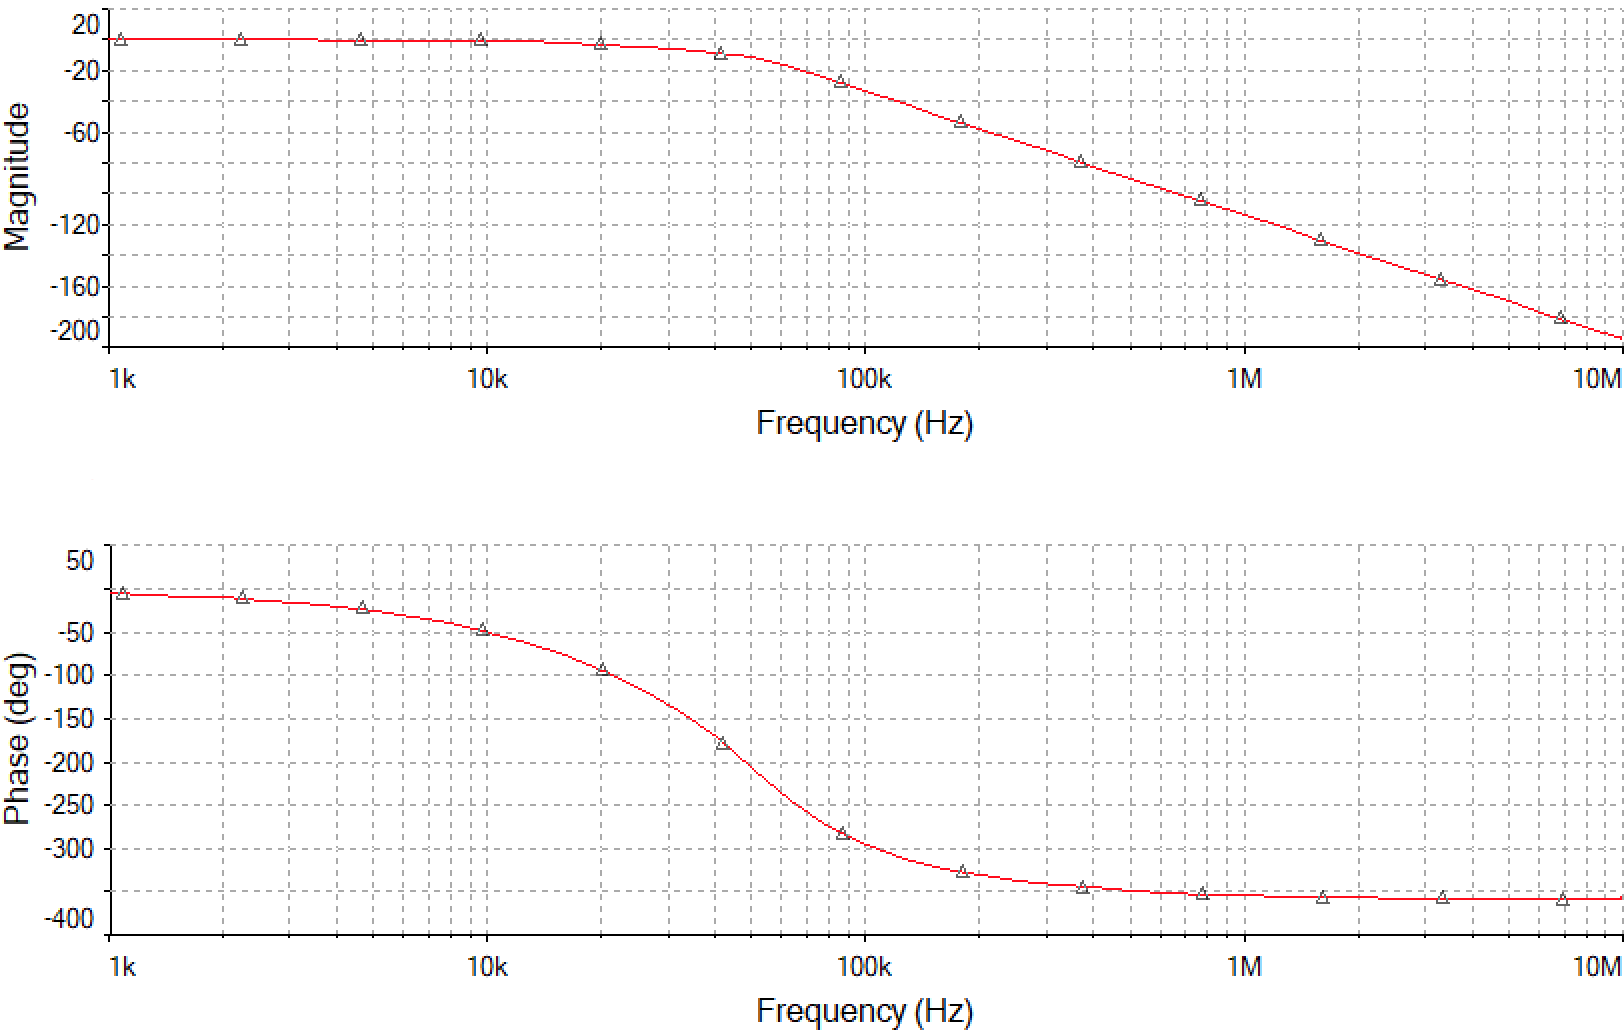
\includegraphics[scale=0.45]{bplp3.png}
\caption{Amplitudová a fázová charakteristika DP 4. řádu}
\end{figure}
\subsection{Pásmová propust 2. řádu}\label{s:PP2}
Horní propust druhého řádu má přenos v nule nulový $H_{0} = 0$. Přenosová funkce je
\begin{align}
H(j\omega) = \frac{H_{\infty} (j\omega) ^2}{(j\omega)^2 + \frac{\omega _c}{Q}(j\omega) + \omega _c ^2}.
\end{align}
\noindent Pásmovou propust lze získat zapojením dolní a horní propusti.
\begin{figure}[H]
\centering
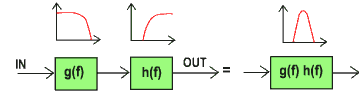
\includegraphics[scale=0.9]{fig9.png}
\caption{Násobení přenosů \cite{13}}
\end{figure}
\noindent Pásmová propust má přenos v nule i nekonečnu nulový $H_{0} = H_{\infty} = 0$. Přenosová funkce je
\begin{align}
H(j\omega) = \frac{H_{B} \frac{\omega _c}{Q} (j\omega) }{(j\omega)^2 + \frac{\omega _c}{Q}(j\omega) + \omega _c ^2}.
\end{align}
\begin{figure}[H]
\centering
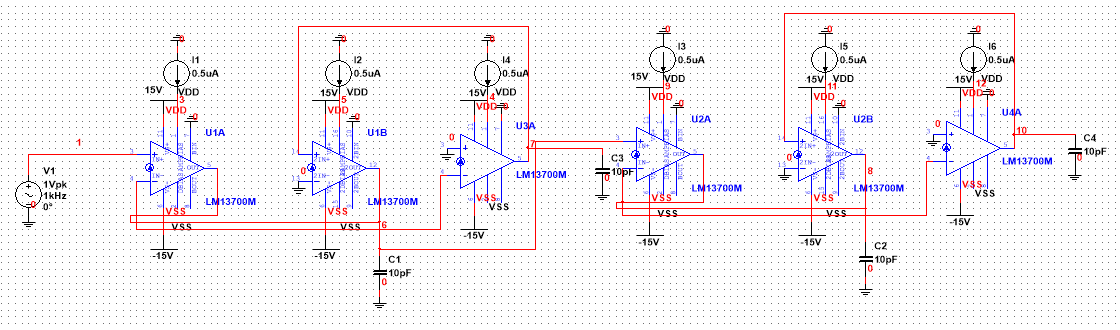
\includegraphics[scale=0.6]{PP2O.png}
\caption{Schéma zapojení PP 2. řádu}
\end{figure}
\begin{figure}[H]
\centering
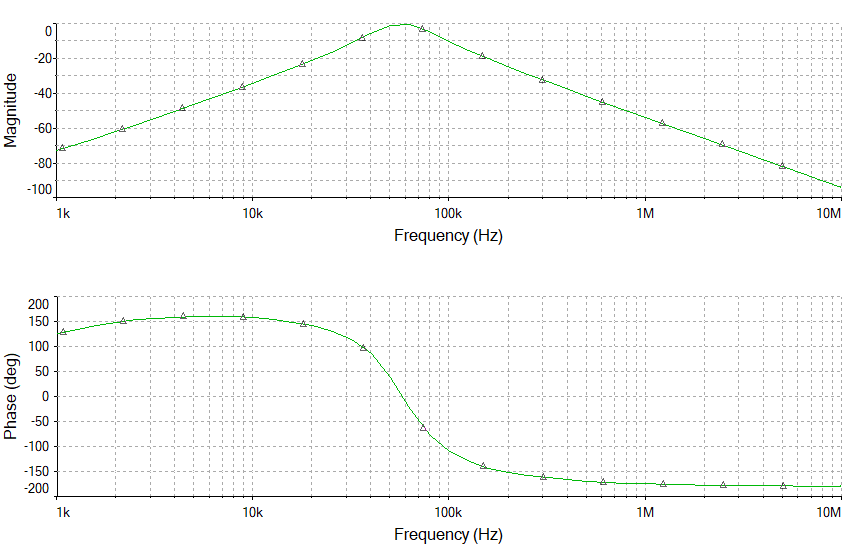
\includegraphics[scale=0.6]{PP2O2.png}
\caption{Amplitudová a fázová charakteristika PP 2. řádu}
\end{figure}
\subsection{Pásmová propust 4. řádu}\label{s:PP4}
\noindent Zapojením dvou PP 2. řádu byla obdržena PP 4.řádu s poklesem -80 dB/dek. 
\begin{figure}[H]
\centering
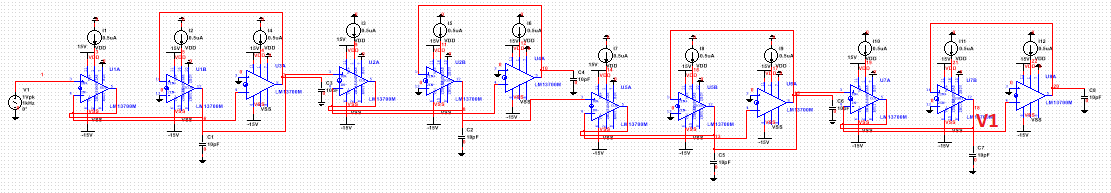
\includegraphics[scale=0.5]{PP4O.png}
\caption{Schéma zapojení PP 4. řádu}
\end{figure}
\begin{figure}[H]
\centering
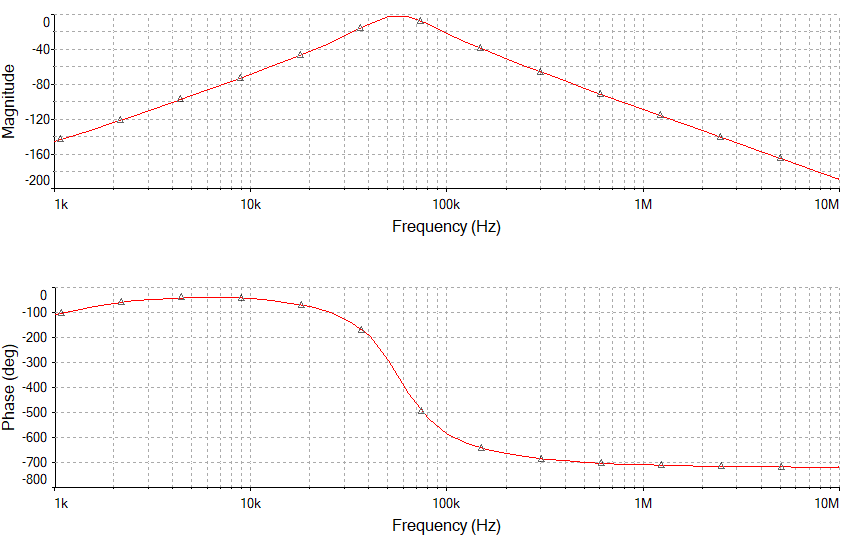
\includegraphics[scale=0.6]{PP4O2.png}
\caption{Amplitudová a fázová charakteristika PP 4. řádu}
\end{figure}
\sekce{Návrh v Maple}\label{s:MAPLE}
Pro návrh pásmové propusti 4. řádu s Cauerovou aproximací typu C byly zvoleny parametry tolerančního schématu 
\MapleOutput{f\_s := 80000 Hz}
\MapleOutput{f\_p := 100000 Hz}
\MapleOutput{fp := 877778 Hz}
\MapleOutput{fs := 100000 Hz}
\MapleOutput{ap := 1 dB}
\MapleOutput{as := 80  dB,}
\noindent kde všechny parametry musí být kladná reálná čísla a f\_s <  f\_p < fp < fs a ap < as. Zadána byla spodní a horní hranice nepropustného pásma $f\_s,fs$ [Hz], spodní a horní hranice propustného pásma $f\_p,fp$ [Hz], maximální útlum v propustném pásmu $ap$ [dB] a minimální útlum v nepropustném pásmu $as$ [dB].
\begin{align}
f\_s &= \frac{\sqrt{\Delta{fs}^2+4f\_m ^2}-\Delta{fs}}{2}\\
f\_p &= \frac{\sqrt{\Delta{fp}^2+4f\_m ^2}-\Delta{fp}}{2}\\
fp &= \frac{\sqrt{\Delta{fp}^2+4f\_m ^2}+\Delta{fp}}{2}\\
fs &= \frac{\sqrt{\Delta{fs}^2+4f\_m ^2}+\Delta{fs}}{2}
\end{align}
Funkcí $BP2NLP$ byla provedena transformace tolerančního schematu nesymetrické pásmové propusti (PP) na toleranční schema normované dolní propusti (NDP). Byl spočten geometrický střed propustného pásma $fm$ [Hz], šířka propustného pásma $\Delta{fp}$ [Hz] a šířka nepropustného pásma $\Delta{fs} $[Hz].
\MapleOutput{fm = 141421 Hz}
\MapleOutput{\Delta{fp} = 100000 Hz}
\MapleOutput{\Delta{fp} = 877778 Hz}
\noindent Byl obdržen kmitočet hranice nepropustného pásma normované dolní propusti (NDP) $Os$ [1/s].
\MapleOutput{Os = 8.77778 1/s}.
\begin{figure}[H]
\centering
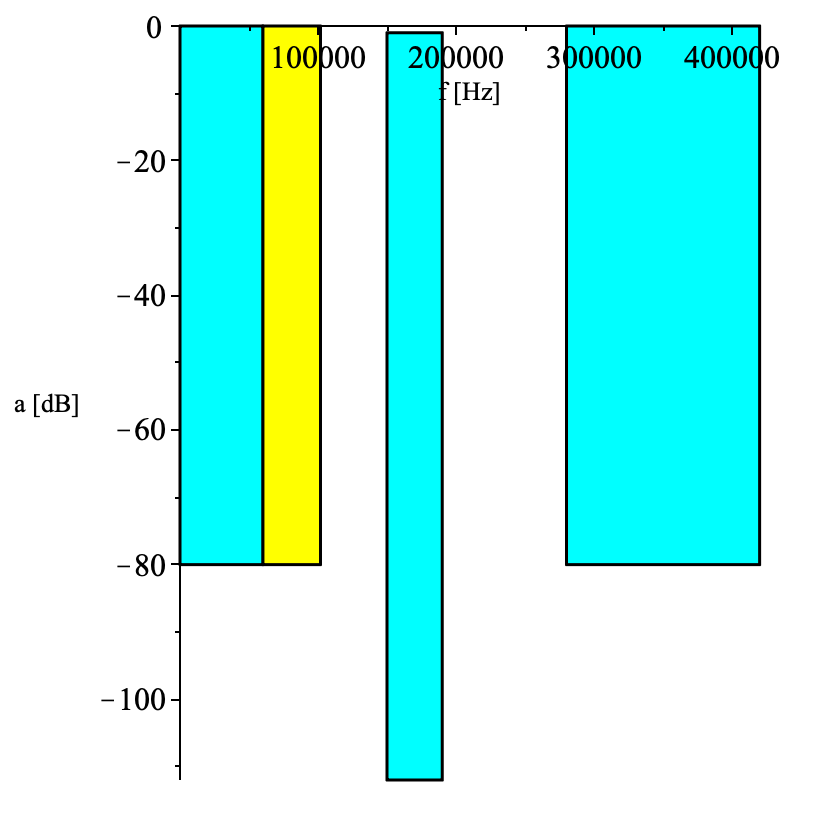
\includegraphics[scale=0.5]{tolsch2.png}
\caption{Toleranční schéma navrhované pásmové propusti}
\end{figure}
\noindent Stupeň Cauerovy aproximace normované dolní propusti byl určen jako $order = 4$.
\noindent Dále byla funkcí $Cauer\_asnew$ určena nová hodnota útlumu v nepropustném pásmu NDP.
\MapleOutput{asnew := 105.613}
\begin{align}
asnew&= 10log10(1 + ( \frac{\epsilon}{kl\_new})^2)\\
\epsilon &= \sqrt{10^{0.1ap} - 1)}\\
k &= \frac{1}{Os}\\
kl\_new &= k^{order}(\prod_{i=1}^{n}JacobiCD(\frac{(2i - 1 + m)EllipticK(k)}{order},k))^4,
\end{align}
\noindent kde $m$ je celočíselný zbytek po dělení řádu 2 a $n$ celočíselný výsledek dělení. Jakobiho eliptických funkcí je 12 a vycházejí ze škálování na jednotkové elipse (cos $\phi$, sin $\phi$ se neváží k jednotkovému kruhu, ale k elipse). $JacobiCD$ funkce je definována jako podíl cosinu Jakobiho funkce s dvěma parametry ($JacobiAM(z,k)$) a derivace této funkce podle prvního parametru z.
\begin{align}
EllipticK(k) = \int _0 ^1(\frac{1}{\sqrt{(-\_ \alpha _1^2+1)}\sqrt{(-k^2 \_ \alpha _1^2+1})})d \_ \alpha _1
\end{align}
Následně byl spočten koeficient nejvyšší mocniny polynomu ve jmenovateli přenosové funkce $Gc$, póly a nuly přenosové funkce $poles, zeros$ pomocí funkce $CauerCPolesZeros$. Počet pólů je dán řádem filtru $order$ a počet nul pro aproximaci typu C je roven $order - 2$. Dále byla spočtena Caurerova aproximace typu C - provozní činitel přenosu $G$ jako racionální lomená funkce $G(j\omega) = 1/H(j\omega)$, charakteristická funkce $chf$ jako $\Phi(j\omega)$ s nulami a póly na imaginární ose a nuly přenosu. Charakteristická funcke má shodný jmenovatel s $G(j\omega)$.
\MapleOutput{Gc, poles, zeros := 376.020,}
\MapleOutput{[-0.475024+0.340009I, -0.475024-0.340009I, -0.162709+0.982758I, -0.162709-0.982758I]),}
\MapleOutput{[11.2840I, -11.2840I],}
\MapleOutput{G,chf,zer := \frac{376.020p^4+479.601p^3+617.689p^2+396.239p+127.328}{p^2+127.329}, \frac{(376.020p^2+311.716)p^2}{p^2+127.329}, [11.2840I, -11.2840I]}
\begin{figure}[H]
\centering
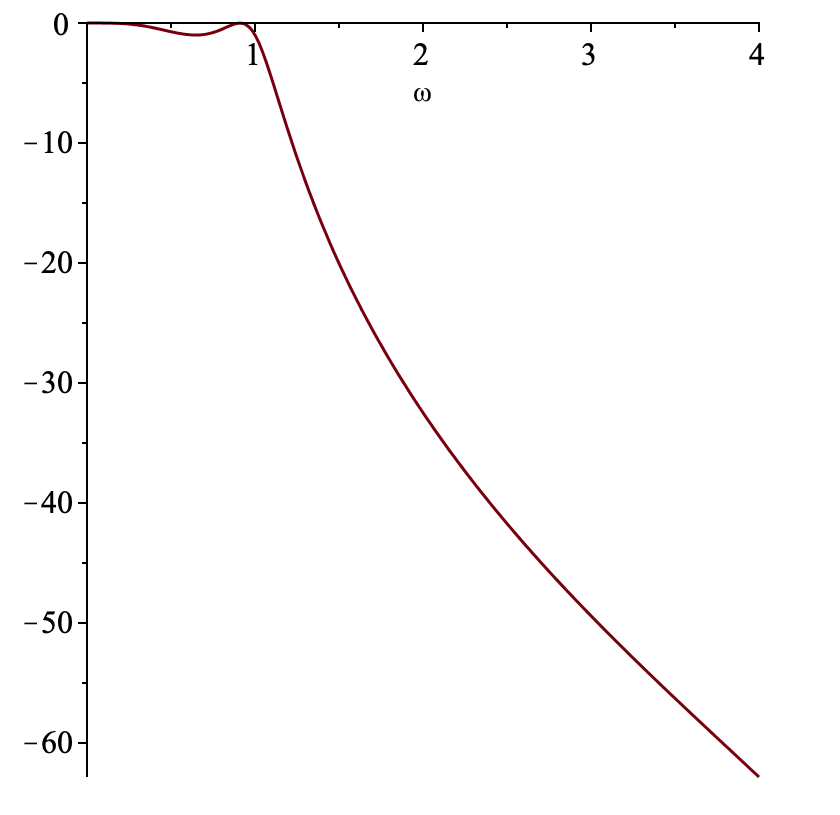
\includegraphics[scale=0.5]{sch02.png}
\caption{Modulová frekvenční charakteristika NDP}
\end{figure}
\noindent Charakteristika byla vykreslena z přenosu funkcí $MagnitudeHdB$, která vypočte modul přenosu podle předpisu |H(j$\omega)$|.
\subsection{Příčkové LC filtry}\label{s:LC}
Pasivní dolní propust je realizována zapojením induktoru ke vstupnímu napětí a k této větvi je následně zapojen paralelně rezistor. Pasivní horní propust má ke vstupu připojený sériově rezistor a poté k této větvi paralelně induktor. \\
K realizaci filtrů vyšších řádů se užívají $\pi$ nebo T články s LC prvky. Při návrhu filtru musí být zohledněn vnitřní odpor zdroje $R_s$ a zatěžovací odpor $R_L$. LC filtry jsou tedy dvojitě zakončeny. Indukčnosti a kapacity prvků se určí z rovnic pro normované kapacity a indukčnosti. Normované hodnoty budou vypočteny pro mezní kmitočet $\omega _c = 1/\sqrt{LC}$ a pro zatěžovací odpor $R_L$. Hodnoty prvků lze pro požadovanou aproximaci odečíst z tabulek. \\
\begin{figure}[H]
\centering
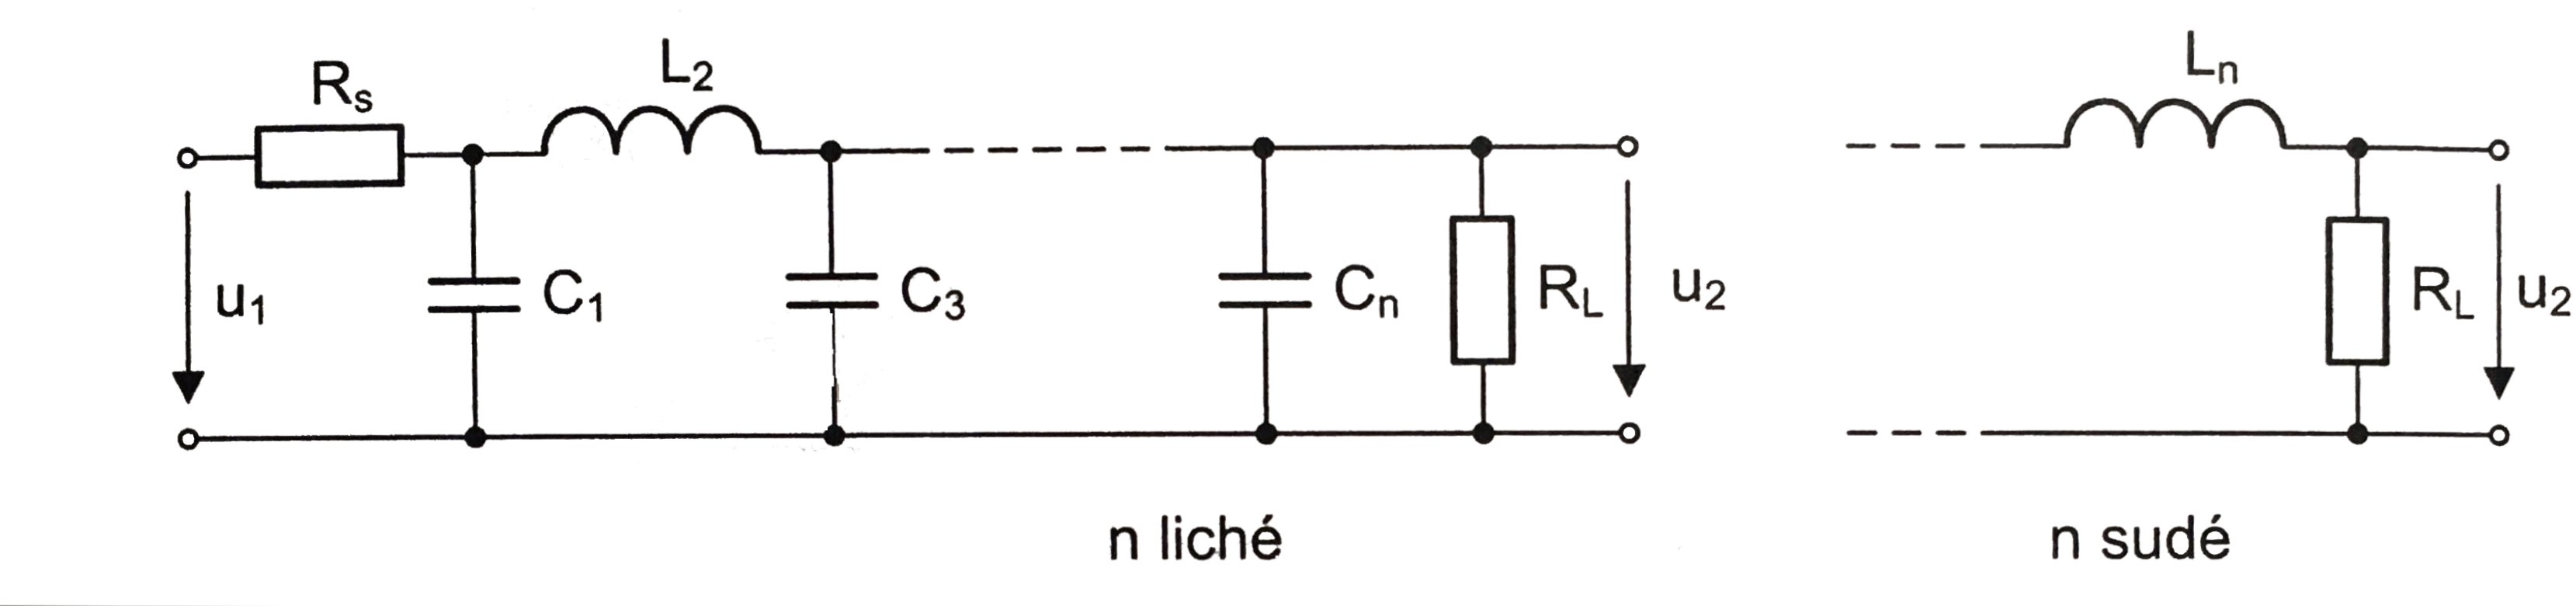
\includegraphics[scale=0.1]{piclanky.png}
\caption{Pasivní dolní propust n-tého řády s $\pi$ články \cite{14}}
\end{figure}
\begin{figure}[H]
\centering
\includegraphics[scale=0.08]{tclanky.png}
\caption{Pasivní dolní propust n-tého řády s T články \cite{14}}
\end{figure}
\newpage
\subsection{Gyrátory}\label{s:GYR}
\noindent K převodu induktoru na zapojení s kapacitorem byla použita struktura označovaná jako gyrátor. Jde o náhradu původního obvodu s induktorem vhodným uspořádáním rezistorů a kapacitorů tak, že výsledná impedance vypadá jako induktor. Gyrátor nelze dobře realizovat s obyčejnými operačními zesilovači, běžně se používají /textit{General Impedance Converters (GIC)}. Převod induktoru na jiné zapojení s ekvivalentní impedancí má praktické využití v integrovaných obvodech, kde jsou kapacitory preferovány nad induktory kvůli malým rozměrům. Gyrátor je principielně spojení invertujícího a neinvertujícího napětím řízeného zdroje proudu, a proto ho lze realizovat snadno s transkonduktančními zesilovači. Na Obrázku \ref{s:GO} jsou znázorněny dva gyrátory s kapacitorem. 
\begin{figure}[H]
\centering
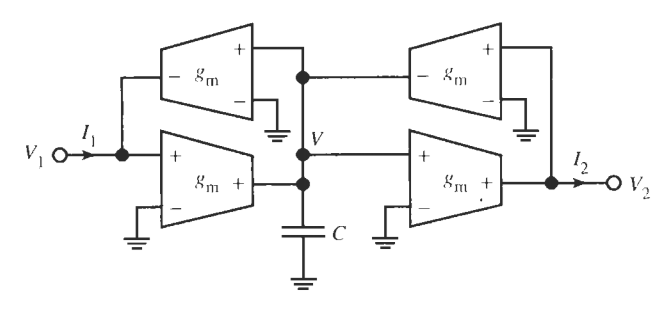
\includegraphics[scale=0.6]{gyrator.png}
\caption{Neuzemněný induktor realizovaný kapacitorem a dvěma gyrátory \cite{12} \label{s:GO}}
\end{figure}
Obvodovou analýzou v uzlu V byla obdržena rovnice
\begin{align}
pCV &= g_mV_1 - g_mV_2
\end{align}
a dva proudy na výstupu
\begin{align}
I_1 = I_2 = g_mV.
\end{align}
Zkombinování rovnic a eliminace V vede k rovnici neuzemněného induktoru mezi napětími $V_1$ a $V_2$.
\begin{align}
I_1 = I_2 = \frac{g_m^2}{pC}(V_1 - V_2) = \frac{1}{pL}(V_1 - V_2)
\end{align}
Z rovnice lze snadno odvodit, že kapacita kondenzátoru použitého při zapojení induktoru s OTA je rovna $C_L = L g_m ^2$. \\
\subsection{Výpočet prvků LC filtru}\label{s:VYP}
\noindent Funkcí $DroppNLP$ byly vypočteny prvky LC příčkového filtru typu normovaná dolní propust (NDP). Zakončení bylo zvoleno standardní (common), odpory o hodnotě 1 $\Omega$, směr zpracování od posledního prvku (rear), s T strukturou (začíná zepředu podélným induktorem). Standardní (common) zakončení je oboustranné ($R_1 \neq 0, R_z \neq \infty$). Výstupem funkce je LC struktura s orientací prvků ve větvi podélně (direct) nebo příčně (shunt).
\MapleOutput{block (1), [orientation = direct, elements = {L1 = -0.40652}, Z = p L1]}
\MapleOutput{block (2), [orientation = shunt, elements = {C1 = 2.4732}, Z = \frac{1}{pC1}]}
\MapleOutput{block (3), [orientation = direct, elements = {C1 = 0.0081309, L1 = 0.96591}, Z = \frac{1}{\frac{1}{pL1} + pC1}]}
\MapleOutput{block (4), [orientation = shunt, elements = {C1 = 1.5489}, Z = \frac{1}{pC1}]}
Vygenerovaná struktura je popsána na Obrázku \ref{s:SCHEM}.
\begin{figure}[H]
\centering
\figppp{Circuit(1)}{5.566}{2.075}{}{}
\caption{Schéma LC příčkové struktury \label{s:SCHEM}}
\end{figure}
\noindent Analýzou LC struktury z Maplu byly obdrženy obvodové rovnice, kde R je volitelný (fiktivní) rezistor:
\begin{align}
I_1 &= \frac{1}{R_1 + pL_1 + \frac{1}{pC_1}}(U_G - U_2)\\
v_1 & = \frac{R}{R_1 + pL_1 + \frac{1}{pC_1}}(U_G - U_2)\\
U_2 &= \frac{1}{\frac{1}{pL_2} + pC_2}(I_1 - I_{3} - I_{L4} - pC_4 v_{L4})\\
U_2 &= \frac{1}{\frac{R}{pL_2} + RpC_2}(v_1 - v_{L3} - v_{L4} - RpC_4 U_{L4})\\
I_{3} &= \frac{1}{pL_3 + \frac{1}{pC_3}}(U_2 - U_3)\\
v_{L3} &= \frac{R}{pL_3 + \frac{1}{pC_3}}(U_2 - U_3)\\
v_{L4} &= \frac{1}{\frac{1}{pL_4}+pC_4}(I_1 - I_{L2} - pC_2U_2 - I_{3} - pC_4 (U_2 - U_3))\\
v_{L4} &= \frac{1}{\frac{R}{pL_4}+RpC_4}(v_1 - v_{L2} - RpC_2U_2 - v_{L3} - RpC_4 (U_2 - U_3))\\
U_3 &= \frac{1}{\frac{1}{R_z}+pC_5 + \frac{1}{pL_5}}(I_1 - I_{L2} - pC_2U_2)\\
U_3 &= \frac{1}{\frac{R}{R_z}+RpC_5 + \frac{R}{pL_5}}(v_1 - U_2 - RpC_2 U_2).
\end{align}
\noindent To odpovídá realizační struktuře s pěti bloky o přenosech $H_1, \ldots,H_5$
\begin{align}
H_1 & = \frac{R}{R_1 + pL_1 + \frac{1}{pC_1}}\\
H_2 &= \frac{1}{\frac{R}{pL_2} + RpC_2}\\
H_3 &= \frac{R}{pL_3 + \frac{1}{pC_3}}\\
H_4 &= \frac{1}{\frac{R}{pL_4}+RpC_4}\\
H_5 &= \frac{1}{\frac{R}{R_z}+RpC_5 + \frac{R}{pL_5}}.
\end{align}
\noindent Uvedené přenosy budou použity v analýze Pracanem.
\noindent Přenosová funkce pasivních a aktivních struktur filtru byla spočtena funkcí $MakeH$. Byl spočten  napěťový i výkonový přenos.
\MapleOutput{H\_NLPV := \frac{p^2  + 127.329}{-193.159 p^4  + 352.072 p^3  + 286.065 p^2  + 582.791 p + 253.653}   }
\MapleOutput{H\_NLP := \frac{p^2  + 127.330}{-96.9631 p^4  + 176.735 p^3  + 143.601 p^2  + 292.553 p + 127.330}}
\begin{figure}[H]
\centering
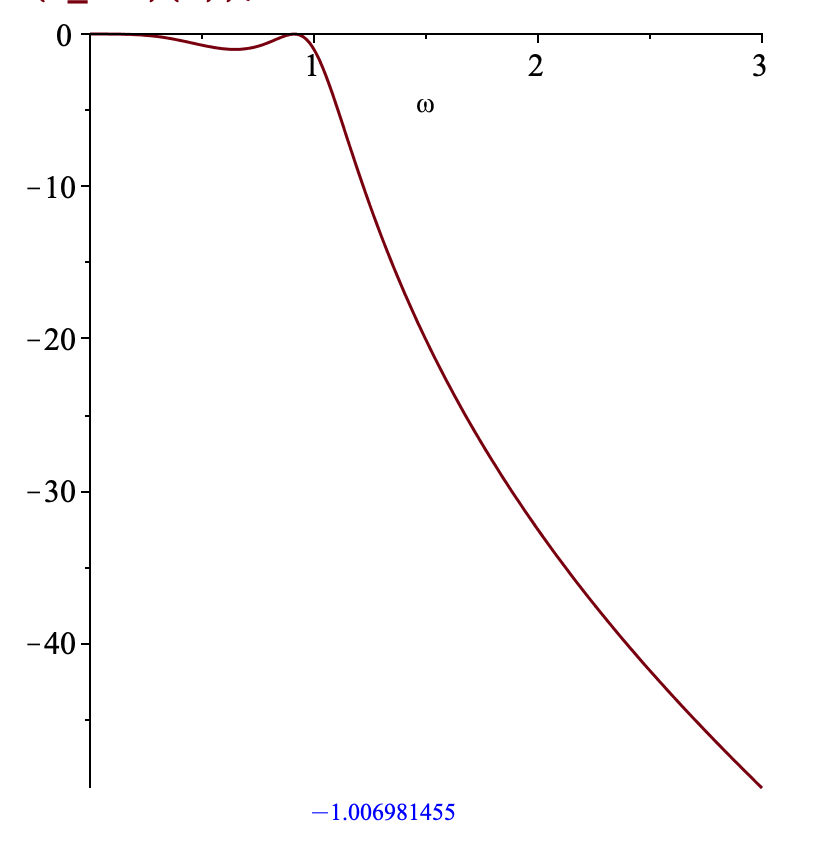
\includegraphics[scale=0.5]{sch022.png}
\caption{Modulová frekvenční charakteristika NDP - LC příčkový filtr}
\end{figure}
\noindent Hodnota přenosové funkce v 1 byla vyhodnocena jako $-2.15882$.\\
Byla provedena transformace hodnot prvků normované dolní propusti (NDP) na pásmovou propust (PP). Zakončovací rezistor byl zvolen 1 $\Omega$, další dva parametry funkce značí spodní a horní hranici propustného pásma.
\MapleOutput{block (1), [Z = p L1 + \frac{1}{pC1}, orientation = direct, elements = { C1 = -7.8301*10^{-6}  , L1 = -3.2350*10^{-7}}]}
\MapleOutput{block (2), [Z = \frac{1}{\frac{1}{pL1}+pC1}, orientation = shunt, elements = {C1 = 1.9681 *10^{-6}, L1 = 1.2871*10^{-6}}]}
\MapleOutput{block (3), [Z = \frac{1}{pC1 + \frac{1}{pL1}+\frac{1}{pL2 + \frac{1}{pC2}}} orientation = direct, elements = { C1 = 6.4704*10^{-9} ,}}
\MapleOutput{C2 = 3.2954*10^{-6}, L1 = 3.9148*10^{-4}, L2 = 7.6864*10^{-7}]}
\MapleOutput{block (4), [Z = \frac{1}{\frac{1}{pL1}+pC1}, orientation = shunt, elements = { C1 = 1.2326 *10^{-6}, L1 = 2.0551*10^{-6}}]}
\noindent Byly nastaveny jakosti cívek v LC příčkové struktuře na konečnou hodnotu. Funkce $MakeRealL$ zařadí do výsledné LC příčkové struktury sériově rezistory k induktorům podle zadaného činitele jakosti $Q$ a zadaného kmitočtu (ten odpovídá u pásmové propusti geometrickému středu propustného pásma - nebo je možno zadat obě hranice propustného pásma). Výpočet sériového odporu je proveden podle předpisu $R_s =L1 \cdot 2 \pi f/Q$.
\MapleOutput{block (1), [Z = p L1 + Rs1 + \frac{1}{pC1}, orientation = direct, elements = { C1 = -7.8301 *10^{-6}, L1 = -3.2350*10^{-7},}}
\MapleOutput{Rs1 = -0.57490*10^{-2}]}
\MapleOutput{block (2), [Z = \frac{1}{\frac{1}{pL1 + Rs1}+pC1}, orientation = shunt, elements = {C1 = 1.9681*10^{-6}, L1 = 1.2871*10^{-6},}}
\MapleOutput{Rs1 = 0.22873*10^{-1}]}
\MapleOutput{block (3), [Z = \frac{1}{pC1 + \frac{1}{pL1 + Rs1}+\frac{1}{pL2 + Rs2 + \frac{1}{pC2}}} orientation = direct, elements = { C1 = 6.4704*10^{-9} ,}}
\MapleOutput{C2 = 3.2954*10^{-6}, L1 = 0.39148*10^{-3}, L2 = 7.6864*10^{-7}, Rs1 = 6.9572, Rs2 = 0.13660*10^{-1}]}
\MapleOutput{block (4), [Z = \frac{1}{\frac{1}{pL1 + Rs1}+pC1}, orientation = shunt, elements = { C1 = 1.2326 *10^{-6}, L1 = 2.0551*10^{-6}, }}
\MapleOutput{Rs1 = 0.36522*10^{-1}]}
\noindent Byl spočten přenos pro LC strukturu bez a s přidanými sériovými rezistory. Pro oba přenosy byla vykreslena modulová frekvenční charakteristika.
\begingroup
    \fontsize{5pt}{12pt}
\MapleOutput{H\_BP := \frac{ p^6  + 2.01858* 10^{14}   p^4  + 1.55854 *10^{23}  p^2}{-6.14026
  10^{-11}  p^8  + 0.000140640 p^7  + 46.6376 p^6  + 5.34196 *10^{8}   p^5 + 2.57033* 10^{14} p^4  + 2.10893 10^{20} p^3  + 7.26886*10^{24} p^2 + 8.65337 *10^{30} p - 1.49149 *10^{36} }}
\MapleOutput{H\_BPQ := \frac{p^7  + 71085.7 p^6 + 2.01860*10^{14}  p^5 + 1.07620*10^{19}p^4+3.47110*10^{23}p^3+6.67244*10^{27}p^2 + 4.92223*10^{31} p}{-6.14027*10^{-11}p^9 +0.000135185 p^8+55.5676 p^7+5.37714*10^8 p^6+2.85360*10^{14} p^5+2.25089*10^{20} p^4+1.49149*10^{25} p^3+8.97641*10^{30} p^2 - 1.38919*10^{36} p - 2.74611*10^{40} }}
\endgroup
\begin{figure}[H]
\centering
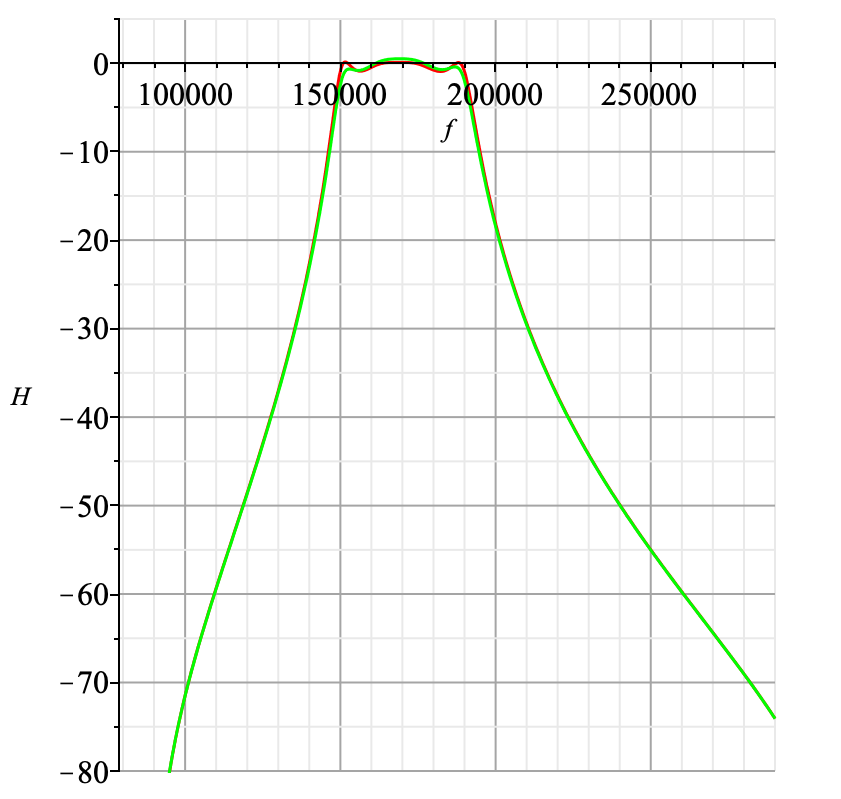
\includegraphics[scale=0.6]{modul12.png}
\caption{Modulová frekvenční charakteristika LC struktury (červená) a LC struktury s konečnou hodntou jakostí cívek (zelená)}
\end{figure}
\noindent Vyčíslením v $200000 \cdot 2 \pi$ Hz byl obdržen útlum 1.21022 dB.\\
\\
\noindent Odnormované prvky byly vyčísleny následovně:
\MapleOutput{ele\_BP := { C1 = -7.83010*10^{-6}  , C2 = 1.96808*10^{-6},  C3 = 3.29545*10^{-6} , C4 = 6.47035*10^{-9},}}
\MapleOutput{ C5 = 1.23258*10^{-6}, L1 = -3.235*10^{-7}, L2 = 1.28706*10^{-6}, L3 = 7.68645*10^{-7}, L4 = 0.391484*10^{-3}, }
\MapleOutput{L5 = 2.05508 *10^{-6}, R1 = 1, Rz = 1.00796}
\noindent Využitím poznatků ze Sekce \ref{s:GYR} byly s uvažováním minimální transkonduktance z datasheetu LM13700 (gm = 9600 $\mu$S) získány kapacity $C_{L1} = 3.08002 $ nF, $C_{L2} = 17.8354$ nF, $C_{L3} = 938.613 $ nF, $C_{L4} = 2.10114$ nF, $C_{L5} = 358.667$ nF.
\noindent Převrácenou hodnotou transkonduktance byly vypočteny frekvenčně a impedančně odnormované odpory
\begin{align}
R_N = R_1 = R_z = \frac{1}{g_m} = 104.16667 \ \Omega.
\end{align}
\noindent Kapacity vyšly již se Syntfilu $C1 = -7.8301 \  \mu$F, $C2 = 1.96808 \  \mu$F, $C3 = 3.29545 \  \mu$F, $C4 = 6.47035$ nF, $C5 = 1.23258 \  \mu$F.
\newpage
\subsection{Návrh funkční simulací}
\noindent  Zapojení s OTA vychází z již uvedených principů v Sekci \ref{s:NAH}. K simulaci byly použity vypočtené hodnoty ze Sekce \ref{s:VYP}. Mezní kmitočet lze přeladit změnou vstupního proudu.
\noindent Bylo použito zapojení se vstupním odporem $R_0$ řazeným paralelně ke zdroji (vhodnější pro funkční simulaci - Schaumann (2001) str. 656/758). Napětí na zdroji poté bude $\frac{V_0}{R_0}$.
\begin{figure}[H]
\centering
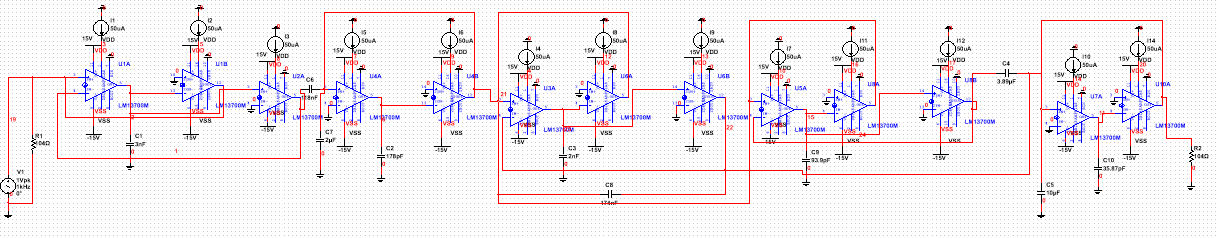
\includegraphics[scale=0.55]{maple.png}
\caption{Výsledné schéma}
\end{figure}
\begin{figure}[H]
\centering
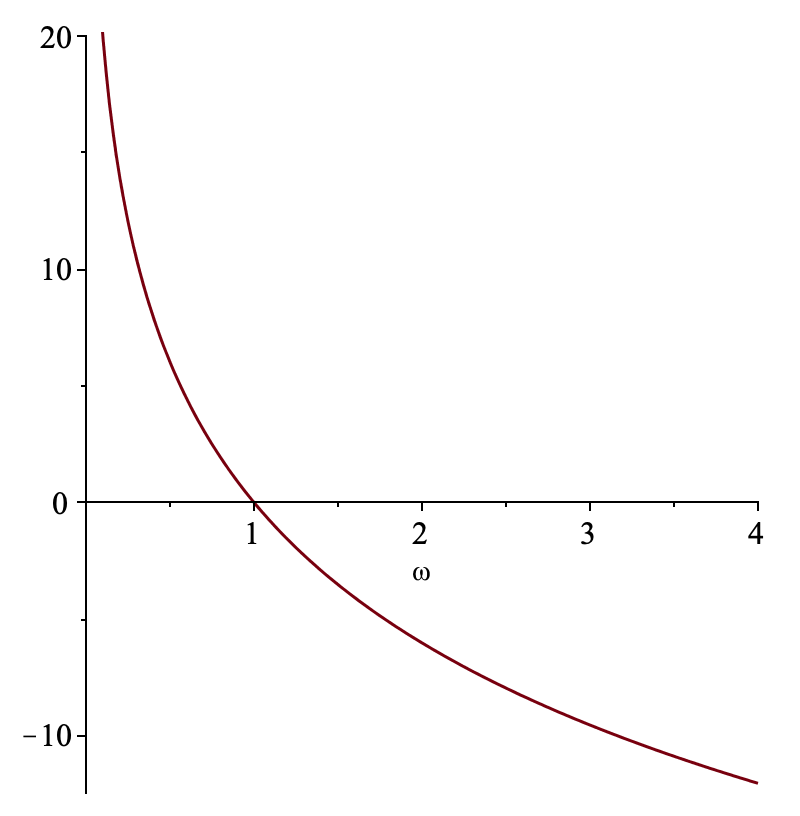
\includegraphics[scale=0.6]{maple2.png}
\caption{Amplitudová a fázová charakteristika PP 4. řádu}
\end{figure}
\sekce{Praktická část}\label{s:PRAK}
\noindent V Altiu byla vytvořena DPS pro DP 4. řádu, PP 2. řádu. Keramický vícevrstvý kapacitor byl zvolen vhodný pro pro povrchovou montáž plošných spojů (SMD) typ C0402C100K56ACAUTO (10~pF, jmenovité napětí stejnosměrného proudu 50~V, tolerance 10~\%). Symboly a footprinty k LM13700M a kapacitoru byly staženy ze~ \url{snapeda.com}. \\
\\
Jako zdroj proudu lze použít NPN tranzistor, nebo operační zesilovač. Různé přístupy k řízení OTA vstupním proudem pomocí napěťového zdroje jsou popsány na obrázku \ref{s:DC} (Geiger, Sanchez-Sinencio \cite{25}). Obrázek a) je nejjednodušší zapojení, ale toto zapojení je velmi citilivé na malé změny napětí. V zapojení b) je řídící napětí uzemněno, ale $V_c$ je citlivé na změny napětí mezi bází a emitorem tranzistoru a na úbytek napětí na diodě. V zapojení c) je řídící napětí také uzemněno a není závislé na součtu nebo vyrušení napětí na pn přechodech. Zenerova dioda je použita k udržení napětí. Frekvenční odezva OZ se zde neuvažuje, protože máme stejnosměrné napětí. Všechna zapojení jsou velmi citlivá na malé změny $V_c$. \\
\\
K řízení odporu byl použit trimmer o hodnotě odporu 1~M$\Omega$. Zapojení se zdrojem na 1~V odpovídá klidový stejnosměrný pracovní proud 1~$\mu$A, který odpovídá dvojnásobku proudu použitého v simulaci. Dle dokumentace k simulačnímu bloku LM13700 je reálný proud dvakrát větší. Trimmer byl zvolen 3361S-1-105GLF (tolerance 10~\%, jmenovitý výkon 500~mW). Schematická značka a footprint s rozměry převzatými z dokumentace byly vytvořeny v Altiu.
\begin{figure}[h]
\centering
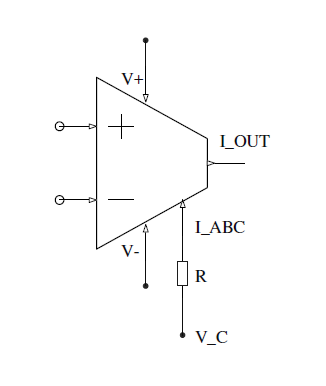
\includegraphics[scale=0.5]{current.png}
\caption{Schéma zapojení napěťového zdroje pro klidový stejnosměrný pracovní proud \label{s:DC}}
\end{figure}
\begin{figure}[h]
\centering
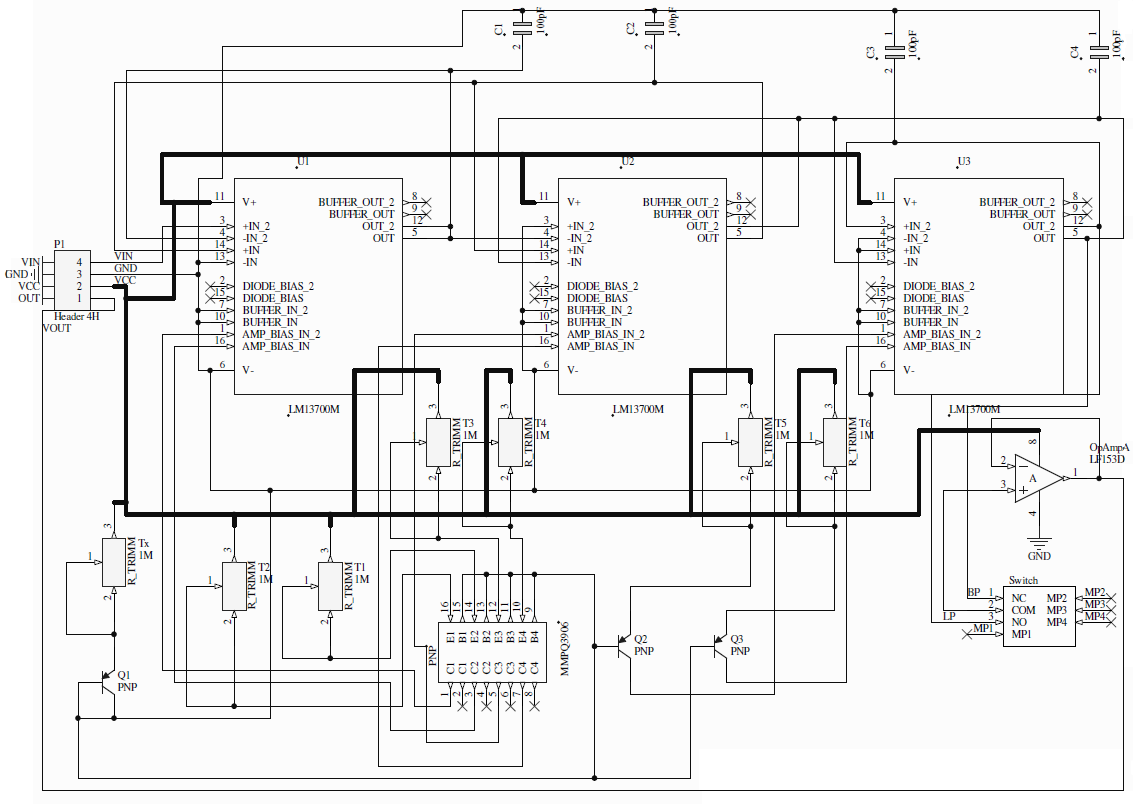
\includegraphics[scale=0.5]{altium.png}
\caption{Schéma obvodu v Altiu}
\end{figure}
\begin{figure}[h]
\centering
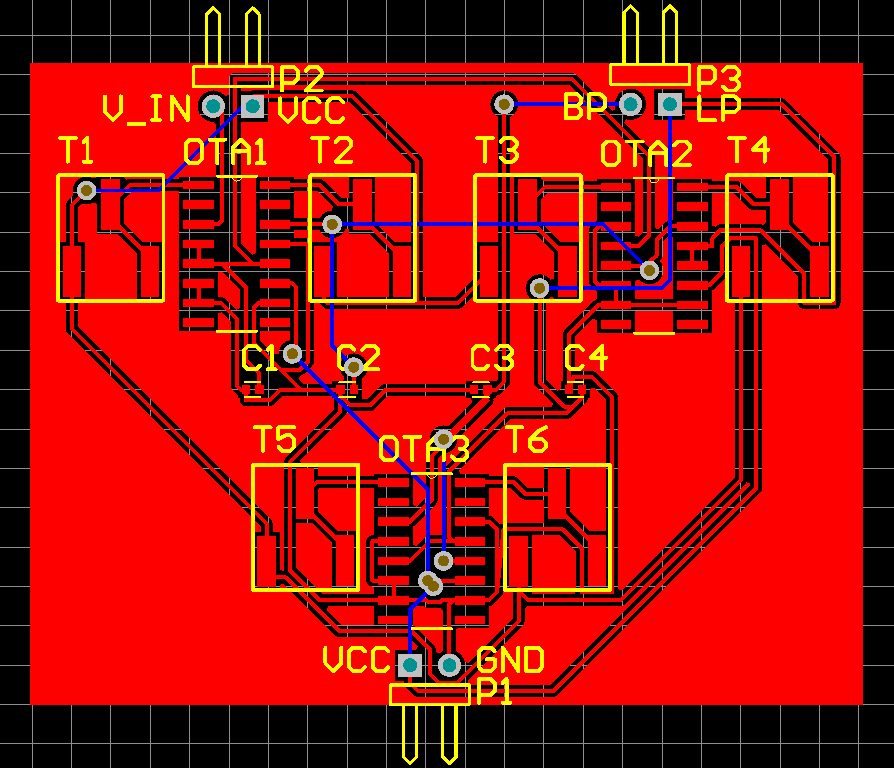
\includegraphics[scale=0.5]{altium2.png}
\caption{PCB layout}
\end{figure}
\sekce{Závěr}
\noindent Cílem práce bylo navrhnout pásmovou propust 4. řádu s Cauerovou aproximací. Po seznámení s principy OTA \ref{s:OTA} a náhradou prvků v obvodech s nimi \ref{s:NAH} byla provedena simulace. V sekci \ref{s:DP2} bylo v MultiSimu realizováno zapojení filtru typu dolní propust 2. řádu s poklesem 40 dB/dek, pásmová propust 1. řádu s poklesem 20 dB/dek. Poté byl kaskádním zapojením obdržen filtr typu dolní propust 4. řádu s poklesem 80 dB/dek, pásmová propust 2. řádu s poklesem 40 dB/dek. Dalším kaskádním blokem byla obdržena požadovaná pásmová propust 4. řádu s poklesem 80~dB/dek. Výsledky simulací prokazují poměrně dobré vlastnosti navržené struktury.\\
\\
V sekci \ref{s:MAPLE} byla knihovnou Syntfil provedena matematická syntéza filtru a zapojení bylo převedeno na LC příčkovou strukturu. Mezní kmitočet a parametry propustného a zádržného pásma byly zvoleny v řádech stovek kHz. Zesílení je možné řídit, stejně tak mezní kmitočet. Mezikrokem v návrhu byl převod pásmové propusti na normovanou dolní propust. Pro LC strukturu byly obdrženy odnormované hodnoty prvků, které byly dosazeny do zapojení s OTA a byla provedena simulace s vypočtenými prvky (sekce \ref{s:SIMAPLE}). Výsledné zapojení ze sekce \ref{s:DP2} obsahovalo 8 kapacitorů. ARC syntézou v sekci \ref{s:ARC}, která spočívá v náhradě indukčností gyrátory, bylo z LC příčkového filtru ze sekce \ref{s:MAPLE} získáno 10 kapacitorů. Kvůli použití pouze rezistorů a kapacitorů jsou filtry realizované kaskádní syntézou výhodnější, protože induktory se musí složitě vyrábět na danou hodnotu. Výsledné schéma celkem obsahuje 12 pasivních a 13 aktivních komponent. V simulaci vycházející z ARC syntézy byl vstupní odpor řazen paralelně ke zdroji. Je nutné dbát na to, že toto zapojení obsahuje neuzemněné kapacity a nebude vhodné pro krátké vlny (frekvence v řádech MHz, což odpovídá vlnovým délkám 10 -- 100~m). Pro tyto vysoké frekvence také OTA nemohou být použity kvůli limitovanému \textit{GBP}. U neuzemněných kapacit je také nutné dbát na to, že vstupní externí proud může způsobit akumulaci náboje na kapacitorech a eventuálně i saturaci OTA. Větší počet OTA také kvůli zpětným vazbám může mít vliv na stabilitu celého obvodu, čímž se sníží pásmo pro vstupní externí proud -- filtr pak může být stabilní jen v malém kmitočtovém pásmu.\\
\\
Dalším krokem byl návrh v KiCadu (sekce \ref{s:PRAK}), praktická realizace a odzkoušení navrhnutého obvodu.\\
Pro lepší návrh by bylo vhodné třeba analyzovat výslednou strukturu popsanou přenosy gyrátorů (sekce \ref{s:MAPLE}) a získat z ní zapojení s OTA, nebo také analyzovat výsledný obvod knihovnou Pracan (schéma struktury lze vyexportovat z KiCadu).
\newpage
\begin{thebibliography}{999}
\bibitem{1}
SHUENN-YUH, Lee a Cheng CHIH-JEN. \textit{Systematic Design and Modeling of a OTA-C Filter for Portable ECG Detection}. IEEE Transactions on Biomedical Circuits and Systems [online]. 2009, Únor 2009 (Vol. 3, no. 1), 11 [cit. 2019-11-05]. Dostupné z: \url{https://www.researchgate.net/publication/224367186_Systematic_Design_and_Modeling_of_a_OTA-C_Filter_for_Portable_ECG_Detection}
\bibitem{2}
\textit{Dlouhé vlny}. Wikipedia: the free encyclopedia [online]. San Francisco (CA): Wikimedia Foundation, 2001- [cit. 2019-11-04]. Dostupné z: \url{https://cs.wikipedia.org/wiki/Dlouh%C3%A9_vlny}
\bibitem{3}
\textit{Střední vlny}. Wikipedia: the free encyclopedia [online]. San Francisco (CA): Wikimedia Foundation, 2001- [cit. 2019-11-04]. Dostupné z: \url{https://cs.wikipedia.org/wiki/St%C5%99edn%C3%AD_vlny}
\bibitem{4}
\textit{ZigBee}. Wikipedia: the free encyclopedia [online]. San Francisco (CA): Wikimedia Foundation, 2001- [cit. 2019-11-04]. Dostupné z: \url{https://cs.wikipedia.org/wiki/ZigBee}
\bibitem{5}
HÁJEK, K., SEDLÁČEK, J. \textit{Kmitočtové  filtry}. Praha, BEN 2002, 536s. ISBN 80-7300-023-7.
\bibitem{6}
SUCHÁNEK, Tomáš. \textit{Kmitočtový filtr} [online]. Brno, 2009 [cit. 2019-11-05]. Dostupné z: \url{https://www.vutbr.cz/www_base/zav_prace_soubor_verejne.php?file_id=17738}. Bakalářská práce. VUT v Brně. Vedoucí práce Ladislav Káňa.
\bibitem{7}
KAŠPER, Ladislav. \textit{Návrh kmitočtového filtru} [online]. Ostrava, 2012 [cit. 2019-04-28]. Dostupné z: \url{https://dspace.vsb.cz/bitstream/handle/10084/92901/KAS279_FEI_N2647_2601T013_2012.pdf?sequence=1&isAllowed=y}. Diplomová práce. VŠB-TU Ostrava, FEI. Strana 18.
\bibitem{8}
RAMSDEN, Ed. \textit{An Introduction to Analog Filters}. Sensors Online [online]. 3 Speen Street, Suite 300, Framingham, MA 01701: Questex, 2019, 1/7/2001 [cit. 2019-05-18]. Dostupné z: \url{https://www.sensorsmag.com/components/introduction-to-analog-filters}
\bibitem{9}
\textit{High-pass filtering pre-processing before computing audio features}. Stack Exchange Inc [online]. 2019 [cit. 2019-04-22]. Dostupné z: \url{https://dsp.stackexchange.com/questions/27586/high-pass-filtering-pre-processing-before-computing-audio-features}
\bibitem{10}
MARTINEK, Pravoslav, Petr BOREŠ a Jiří HOSPODKA. \textit{Elektrické filtry}. Praha: Vydavatelství ČVUT, 2003. ISBN 80-01-02765-1. Strana 74, obrázek 4.17. Strana 141, obrázek 5.43.
\bibitem{11}
MICHAL, Vratislav. \textit{Vybrané vlastnosti obvodů pracujících v proudovém módu a napěťovém módu} [online]. Brno, 2017 [cit. 2019-03-30]. Dostupné z: \url{https://docplayer.cz/43256146-Vybrane-vlastnosti-obvodu-pracujicich-v-proudovem-modu-a-napetovem-modu.html}. Článek. Brno University of Technology. Strana 5.
\bibitem{12}
HOSPODKA, Jiří. \textit{Úvod do analogových filtrů} [online]. Praha, 2018 [cit. 2019-03-30]. Dostupné z: \url{https://moodle.fel.cvut.cz/course/view.php?id=1434}. Přednáška. ČVUT FEL. Strana 21, 24.
\bibitem{13}
SMITH, K.C., SEDRA, A.S. \textit{The current conveyor: a new circuit building block}. New York, 1968 (Vol. 56, no. 3). Článek. IEEE Proc. Strana 1368--1369.
\bibitem{14}
SMITH, K.C., SEDRA, A.S. \textit{A second generation current conveyor and its application}. New York, 1970 (CT-17). Článek. IEEE Trans. Strana 132--134.
\bibitem{15}
SHAKTOUR, Mahmoud. \textit{Nekonvenční obvodové prvky pro návrh příčkových filtrů} [online]. Brno, 2010 [cit. 2019-10-25]. Dostupné z: \url{https://www.vutbr.cz/www_base/zav_prace_soubor_verejne.php?file_id=35975}. Disertační práce. Vysoké učení technické v Brně. Vedoucí práce Dalibor Biolek. Strana 8, obrázek 3-1 (a). Strana 9, obrázek 3-2. Strana 11, obrázek 3--5. Strana 12, obrázek 3-6.
\bibitem{16}
\textit{Transconductance Amplifiers} [online]. 2019 [cit. 2019-03-30]. Dostupné z: \url{https://cz.mouser.com/Semiconductors/Integrated-Circuits-ICs/Amplifier-ICs/Transconductance-Amplifiers/_/N-6j73l?P=1y95od0}
\bibitem{17}
LM13700: Dual Operational Transconductance Amplifiers With Linearizing Diodes and Buffers. In: \textit{Texas Instruments} [online]. Dallas, Texas: Texas Instruments Incorporated, 2018 [cit. 2019-03-30]. Dostupné z: \url{www.ti.com/lit/ds/symlink/lm13700.pdf} Strana 1. Strana 9, obrázek 16.
\bibitem{18}
SCHAUMANN, Rolf a Mac E. Van VALKENBURG. \textit{Design of Analog Filters}. New York: Oxford University Press, 2001. ISBN 0195118774. Strana 213, obrázek 4-13. Strana 236, obrázek 4-35 a),b). Strana 237, obrázek 4-36 a),b). Strana 608, obrázek 16-2 a),b).
\renewcommand{\headrulewidth}{0pt}
\fancyhf{}
\bibitem{19}
VEDRAL, Josef a Jakub SVATOŠ. \textit{Zpracování a digitalizace analogových signálů v měřící technice}. Praha: Česká technika - nakladatelství ČVUT, 2018. ISBN 978-80-01-06424-5. Strana 136, obrázek 5.3.9, 5.3.10.
\bibitem{20}
MOTCHENBACHER, C. D.; CONNELLY, J. A. \textit{Low-noise electronic system design}. [s.l.]: Wiley Interscience, 1993.
\bibitem{21}
\textit{Elektronický šum}. In: Wikipedia: the free encyclopedia [online]. San Francisco (CA): Wikimedia Foundation, 2001- [cit. 2019-11-05]. Dostupné z: \url{https://cs.wikipedia.org/wiki/Elektronick%C3%BD_%C5%A1um#cite_note-noise-1}
\bibitem{22}
GEIGER, Randall L. a Edgar SÂNCHEZ-SINENCIO. \textit{Active Filter Design Using Operational Transconductance Amplifiers: A Tutorial}. IEEE CIRCUITS AND DEVICES MAGAZINE [online]. 1985, 1985 (Březen), 13 [cit. 2019-11-06]. Dostupné z: \url{https://www.ece.uic.edu/~vahe/spring2013/ece412/OTA-structures2.pdf}
\bibitem{23}
\textit{THD}. In: Wikipedia: the free encyclopedia [online]. San Francisco (CA): Wikimedia Foundation, 2001- [cit. 2019-11-19]. Dostupné z: \url{https://cs.wikipedia.org/wiki/THD}
\bibitem{24}
\textit{SNR poměr}. In: Optixs.cz [online]. Praha, 2019 [cit. 2019-11-19]. Dostupné z: \url{https://www.optixs.cz/slovnik-17/snr-pomer-70s}
\bibitem{25}
\textit{Signal-to-noise ratio}. In: Wikipedia: the free encyclopedia [online]. San Francisco (CA): Wikimedia Foundation, 2001- [cit. 2019-11-19]. Dostupné z: \url{https://en.wikipedia.org/wiki/Signal-to-noise_ratio}
\end{thebibliography}
\renewcommand{\headrulewidth}{0pt}
\fancyhf{}
\nadpis{Seznam přiložených souborů na CD}
\begin{figure}[H]
	\dirtree{%
		.1 readme.txt\DTcomment{soubor s popisem obsahu CD}.
		.1 Altium\DTcomment{adresář se schématem DPS}.
		.2 Assembly Drawings.pdf\DTcomment{schéma DPS pouze se součástkami}.
		.2 Composite Drill Drawing.pdf\DTcomment{schéma pro vrtání}.
		.2 Final Artwork Prints.pdf\DTcomment{soubor se všemi vrstvami na desce}.
		.2 Libraries\DTcomment{adresář s knihovnami}.
		.2 PCB Prints.pdf\DTcomment{schéma DPS}.
		.2 Schematic Prints.pdf\DTcomment{schéma zapojení}.
		.2 Solder\_Paste Mask Prints.pdf\DTcomment{schéma pro vrstvu pájecí pasty}.
		.1 Altium biquads\DTcomment{schémata a DPS pro různá zapojení bikvadů}.
		.1 Doc\DTcomment{dokumentace}.
		.2 lm13700.pdf\DTcomment{datasheet k LM13700}.
		.1 Images\DTcomment{obrázky použité v textu}.
		.1 LaTeX\DTcomment{adresář s \LaTeX{} zdrojovými kódy}.
		.1 Maple\DTcomment{adresář s Maple skripty}.
		.2 bandpass\_cauer.mw\DTcomment{Cauerova aproximace}.
		.2 bandpass\_butterworth.mw\DTcomment{Butterworthova aproximace}.
		.2 bandpass\_chebyshev.mw\DTcomment{Chebyshevova aproximace}.
		.1 Multisim\DTcomment{soubory se schématy v Multisimu}.
		.2 BP4.ms14 \DTcomment{pásmová propust 4. řádu}.
		.2 BPLPHP.ms14 \DTcomment{základní zapojení pro bikvad}.
		.2 butterworth\_highpass.ms14 \DTcomment{Butterworthova aproximace HP 2. řádu}.
		.2 highpass\_rc.ms14 \DTcomment{horní propust 1. řádu}.
		.2 LP2.ms14 \DTcomment{dolní propust 2. řádu}.
		.2 LP4BP2.ms14 \DTcomment{dolní propust 4. řádu, pásmová propust 2. řádu}.
		.2 MapleOutput\_butterworth.ms14 \DTcomment{Butterworthova aproximace PP 4. řádu}.
		.2 MapleOutput\_butterworth2.ms14 \DTcomment{Butterworthova aproximace PP 4. řádu}.
		.2 MapleOutput\_cauer.ms14 \DTcomment{Cauerova aproximace PP 4. řádu}.
		.1 Thesis Text\DTcomment{adresář s textem práce}.
		.2 BP\_Pacalova\_Klara\_2020.pdf\DTcomment{práce v PDF formátu}.
	}
\end{figure}
\end{document}
